\section{Analysis}
\begin{justify}
    The following section will contain the Analysis Phase of the Software Development Life Cycle of Student Talent Development Center: Design and Implementation of Scheduling and Resources Management Web Application System.\\
\end{justify}


\subsection{Requirement Elicitation (Requirements Gathering)}
\begin{justify}
    The Student Talent Development Center of the University of Kurdistan Hewlêr offers a variety of services to assist its students in succeeding, including Peer Assisted Learning (PAL), Wellbeing \& Counseling, and Personal Academic Tutors. The followings are the requirements gathered from the stakeholders of the project for the center's Peer Assisted Learning subcenter. The below scenario demonstrates what the stakeholders are looking for.

    \vspace{0.25cm}
    \newendline \textbf{Scenario}

    \noindent As a student at the University of Kurdistan Hewlêr, Sarkazh logs into the Student Talent Development Center (STDC) web application using his UKH email and password. He is immediately presented with a list of courses that are currently being taught in the STDC, with his current courses appearing at the top. He clicks on the course "Introduction to Programming" to view more details about it. He also notices that the upcoming lesson's time and venue are displayed when he views the session. He remembers that he has attended this session before, so he clicks on the "History" button to view past sessions he has attended.\newendline
    Sarkazh sees that there is an upcoming session for the "Introduction to Programming" course, so he clicks on the "Register" button to sign up for it. He also sees that there are materials uploaded for the sessions he has attended, so he clicks on the "Materials" button to view them. \newendline
    Meanwhile, Didam, one of the tutors at the STDC, logs into the web application using her UKH email and password. She is responsible for teaching the "Introduction to Programming" course, so she clicks on the "Sessions" button to view the list of sessions she is teaching. She sees that Sarkazh has registered for the upcoming session, so she clicks on the "Students" button to view the list of students who have registered for it. She also sees that she has to enter the attendance of the previous session, so she clicks on the "Attendance" button to do so.\newendline
    Didam remembers that she has another class at the same time as the upcoming session, so she clicks on the "Availability" button to update her schedule. She also sees that she has to upload materials for the session, so she clicks on the "Materials" button to upload the files. She also sees that she has already taught for 15 hours, which is displayed on her profile.\newendline
    Finally, the admin at the STDC, Ranj, logs into the web application using his UKH email and password. He is responsible for managing the courses, sessions, venues and tutors at the STDC. He clicks on the "Courses" button to view the list of courses currently being taught at the STDC. He sees that he needs to create a new course, so he clicks on the "Create" button to do so. He also sees that he needs to update an existing course, so he clicks on the "Update" button to do so. He also sees that he needs to delete an existing course, so he clicks on the "Delete" button to do so. \newendline
    Ranj also clicks on the "Sessions" button to view the list of sessions currently being held at the STDC. He sees that he needs to create a new session, so he clicks on the "Create" button to do so. He also sees that he needs to update an existing session, so he clicks on the "Update" button to do so. He also sees that he needs to delete an existing session, so he clicks on the "Delete" button to do so. \newendline
    Ranj also clicks on the "Venues" button to view the list of venues currently available at the STDC. He sees that he needs to create a new venue, so he clicks on the "Create" button to do so. He also sees that he needs to update an existing venue, so he clicks on the "Update" button to do so. He also sees that he needs to delete an existing venue, so he clicks on the "Delete" button to do so. \newendline
    Finally, Ranj clicks on the "Tutors" button to view the list of tutors currently working at the STDC. He sees that he needs to onboard a new tutor, so he clicks on the "Onboard" button to do so. He also sees that he needs to assign a tutor to a course, so he clicks on the "Assign" button to do so. He also sees that he needs to list the attendance of a session using the specified button. He also clicks on the "Feedback" button to view the student feedbacks and view individual feedback.    


    \newendline\textbf{Requirement Categorization and Prioritization}\\
    Each requirement below is categorized and prioritized base on the following format: 
    \begin{itemize}
        \definecolor{vin}{RGB}{180,9,39}
        \item \textbf{\textit{System Component}}
            \begin{itemize}
                \item MoSCoW Priority
                    \begin{itemize}
                        \item \textbf{\textcolor{vin}{Associated Requirement ID}} -- Use Case Name -- Actor.\\Brief Description.
                    \end{itemize}
            \end{itemize}
    \end{itemize}

    \noindent It is also worth mentioning that the following requirement are the requirements that will be used and refereed to as a reference of the system's whole functional requirements. The unique associated requirement ids are used throughout the project to reference a specific requirement.\newendline
    
    \begin{itemize}
        \definecolor{vin}{RGB}{180,9,39}
        \item \textbf{\textit{System Core}}
            \begin{itemize}
                \item Must Have
                    \begin{itemize}
                        \item \textbf{\textcolor{vin}{RQ01}} -- Login -- All Users.\\All users must be able to login using UKH email and Password.
        
                        \item \textbf{\textcolor{vin}{RQ02}} -- Enter Attendance -- Tutor.\\Tutor must be able to enter attendance of each session.

                        \item \textbf{\textcolor{vin}{RQ03}} -- List Courses -- All Users.\\All users must list courses taught in STDC. (Current User’s courses should appear on top).
                        
                        \item \textbf{\textcolor{vin}{RQ04}} -- View Course -- All Users.\\All users must be able to view an individual course.

                        \item \textbf{\textcolor{vin}{RQ05}} -- Create Course -- Admin.\\Admin must be able to create a new course.

                        \item \textbf{\textcolor{vin}{RQ06}} -- Update Course -- Admin.\\Admin must be able to update a course.

                        \item \textbf{\textcolor{vin}{RQ07}} -- Delete Course -- Admin.\\Admin must be able to delete a course.

                        \item \textbf{\textcolor{vin}{RQ08}} -- List Sessions -- All Users.\\All users must be able to list sessions.
                        
                        \item \textbf{\textcolor{vin}{RQ09}} -- View Session -- All Users.\\All users must be able to view an individual session.

                        \item \textbf{\textcolor{vin}{RQ10}} -- Create Session -- Admin.\\Admin must be able to create a new session.

                        \item \textbf{\textcolor{vin}{RQ11}} -- Update Session -- Admin.\\Admin must be able to update an existing session.

                        \item \textbf{\textcolor{vin}{RQ12}} -- Delete Session -- Admin.\\Admin must be able to delete an existing session.

                        \item \textbf{\textcolor{vin}{RQ13}} -- List Venues -- Admin.\\Admin must be able to list venues.
                        
                        \item \textbf{\textcolor{vin}{RQ14}} -- View Venue -- All Users.\\All users must be able to view an individual venue.

                        \item \textbf{\textcolor{vin}{RQ15}} -- Create Venue -- Admin.\\Admin must be able to create (register) a new venue.

                        \item \textbf{\textcolor{vin}{RQ16}} -- Update Venue -- Admin.\\Admin must be able to update an existing venue.

                        \item \textbf{\textcolor{vin}{RQ17}} -- Delete Venue -- Admin.\\Admin must be able to delete an existing venue.

                        \item \textbf{\textcolor{vin}{RQ18}} -- Onboard Tutor -- Admin.\\Admin must be able to onboard tutors.

                        \item \textbf{\textcolor{vin}{RQ19}} -- Assign Tutor -- Admin.\\Admin must be able to assign tutors courses.
                        
                    \end{itemize}
                    
                \item Should Have
                    \begin{itemize}
                        \item \textbf{\textcolor{vin}{RQ20}} -- View Attendance -- Admin.\\Admin and Tutor should be able to list the attendance of a session using specified button.

                        \item \textbf{\textcolor{vin}{RQ32}} -- View Profile -- All Users.\\All users should be able to view their profile and its details.
                    \end{itemize}
            \end{itemize}
            
        \item \textbf{\textit{Scheduling System}}
            \begin{itemize}
                \item Must Have
                    \begin{itemize}
                        \item \textbf{\textcolor{vin}{RQ21}} -- View Time and Venue -- All Users.\\All users must see upcoming lesson’s time and venue when they view a session.
                        
                        \item \textbf{\textcolor{vin}{RQ22}} -- Assign Time and Venue -- Admin.\\Admin must be able to assign time and venue to each session.
                    \end{itemize}
                    
                \item Should Have
                    \begin{itemize}
                        \item \textbf{\textcolor{vin}{RQ23}} -- View History -- Student \& Tutor.\\Student and Tutor should see the history of sessions they have attended.

                        \item \textbf{\textcolor{vin}{RQ24}} -- Enter Availability -- Tutor.\\Tutor should be able to enter their availability.
                        
                        \item \textbf{\textcolor{vin}{RQ33}} -- Register for Session -- Student.\\Students should be able to register for upcoming session.

                        \item \textbf{\textcolor{vin}{RQ34}} -- View Registered Students -- Tutor.\\Tutor should be able to view students who have registered for upcoming session.
                    \end{itemize}
                    
                \item Could Have
                    \begin{itemize}
                        \item \textbf{\textcolor{vin}{RQ25}} -- Cancel Session -- Tutor.\\Tutor could cancel a session.

                        \item \textbf{\textcolor{vin}{RQ26}} -- View Hours -- Admin \& Tutor.\\Admin and Tutor could see how many hours tutor have tutored when viewing tutor profile.
                    \end{itemize}
            \end{itemize}
        \item \textbf{\textit{Feedback System}}
            \begin{itemize}
                \item Should Have
                    \begin{itemize}
                        \item \textbf{\textcolor{vin}{RQ27}} -- Provide Feedback -- Student.\\Student should be able to provide feedback after each session.

                        \item \textbf{\textcolor{vin}{RQ28}} -- View Feedbacks -- Admin.\\Admin should be able to list student feedbacks.

                        \item \textbf{\textcolor{vin}{RQ31}} -- View Feedback -- Admin.\\Admin should be able to view student feedback individually.

                        \item \textbf{\textcolor{vin}{RQ35}} -- List Questions -- Admin.\\Admin must be able to list questions.
                        
                        \item \textbf{\textcolor{vin}{RQ36}} -- View Question -- All Users.\\All users must be able to view an individual question.

                        \item \textbf{\textcolor{vin}{RQ37}} -- Create Question -- Admin.\\Admin must be able to create (register) a new question.

                        \item \textbf{\textcolor{vin}{RQ38}} -- Delete Question -- Admin.\\Admin must be able to delete an existing question.
                    \end{itemize}
            \end{itemize}
        \item \textbf{\textit{Resources System}}
            \begin{itemize}
                \item Should Have
                    \begin{itemize}
                        \item \textbf{\textcolor{vin}{RQ29}} -- Access Material -- All Users.\\All users should be able to access materials uploaded.

                        \item \textbf{\textcolor{vin}{RQ30}} -- Upload Material -- Tutor.\\Tutors should be able to upload files (material) for a given session of a course.\\
                    \end{itemize}
            \end{itemize}
    \end{itemize}

    \clearpage
    \newendline \textbf{Further Constraints to Functional Requirements}
    \begin{itemize}
        \item Students won’t be able to provide feedback for sessions older than a week.
        \item Students won’t be able to provide feedback to sessions they have not participated in.
        \item Students must see the material uploaded only for sessions that they have attended.
        \item Tutors upload files to sessions which belongs to a course.\newendline
    \end{itemize}

    \noindent \textbf{Non-Functional Requirements}
    \begin{itemize}
        \item Performance
            \begin{itemize}
                \item The ability to have concurrent users on our web application.
                \item Each request should be processed within no more than 5 seconds.
            \end{itemize}
        \item Security
            \begin{itemize}
                \item To keep the system secure, standard encryption methods such as RS256 will be used.
                \item Implementing OAuth 2.0 and OpenID connect to keep the system secure.
                \item Using Json Web Token (JWT) to keep sessions and to have secure up to date security standards.
            \end{itemize}
        \item Reliability
            \begin{itemize}
                \item System can fail no more than 3 hours per year.
            \end{itemize}
        \item Usability
            \begin{itemize}
                \item The users can easily determine what a feature is and what it can do. E.g. clicking on a button with an icon of a magnifier should open search bar.\\
            \end{itemize}
    \end{itemize}
\end{justify}

\clearpage

\subsection{Requirement Specification}
\begin{justify}
The following is the Analysis phase's Requirement Specifications document. In this phase, requirements are analyzed using Use Cases and Activity Models. The analysis is done using the following tools:
\begin{enumerate}
    \item UML Use Case Model
    \item Use Case Tabular Form
    \item UML Activity Model
\end{enumerate}

\noindent Four elements compose the Student Talent Development Center Web Application. The System Core, Scheduling System, Feedback System, and Resource Management System. These four components are formed based on the requirements above.

\newendline Microsoft Azure Business-to-Consumer (B2C) Identity Server interacts with the System despite the fact that it has four internal components. This external component is integrated but not a part of the system. It provides security and abstraction to user management concerns.

\clearpage
\vspace{0.25cm}
\newendline\textbf{UML Use Case Model}\\
The following are the use case models of each component of the system.

\begin{figure}[H]
    \centerline{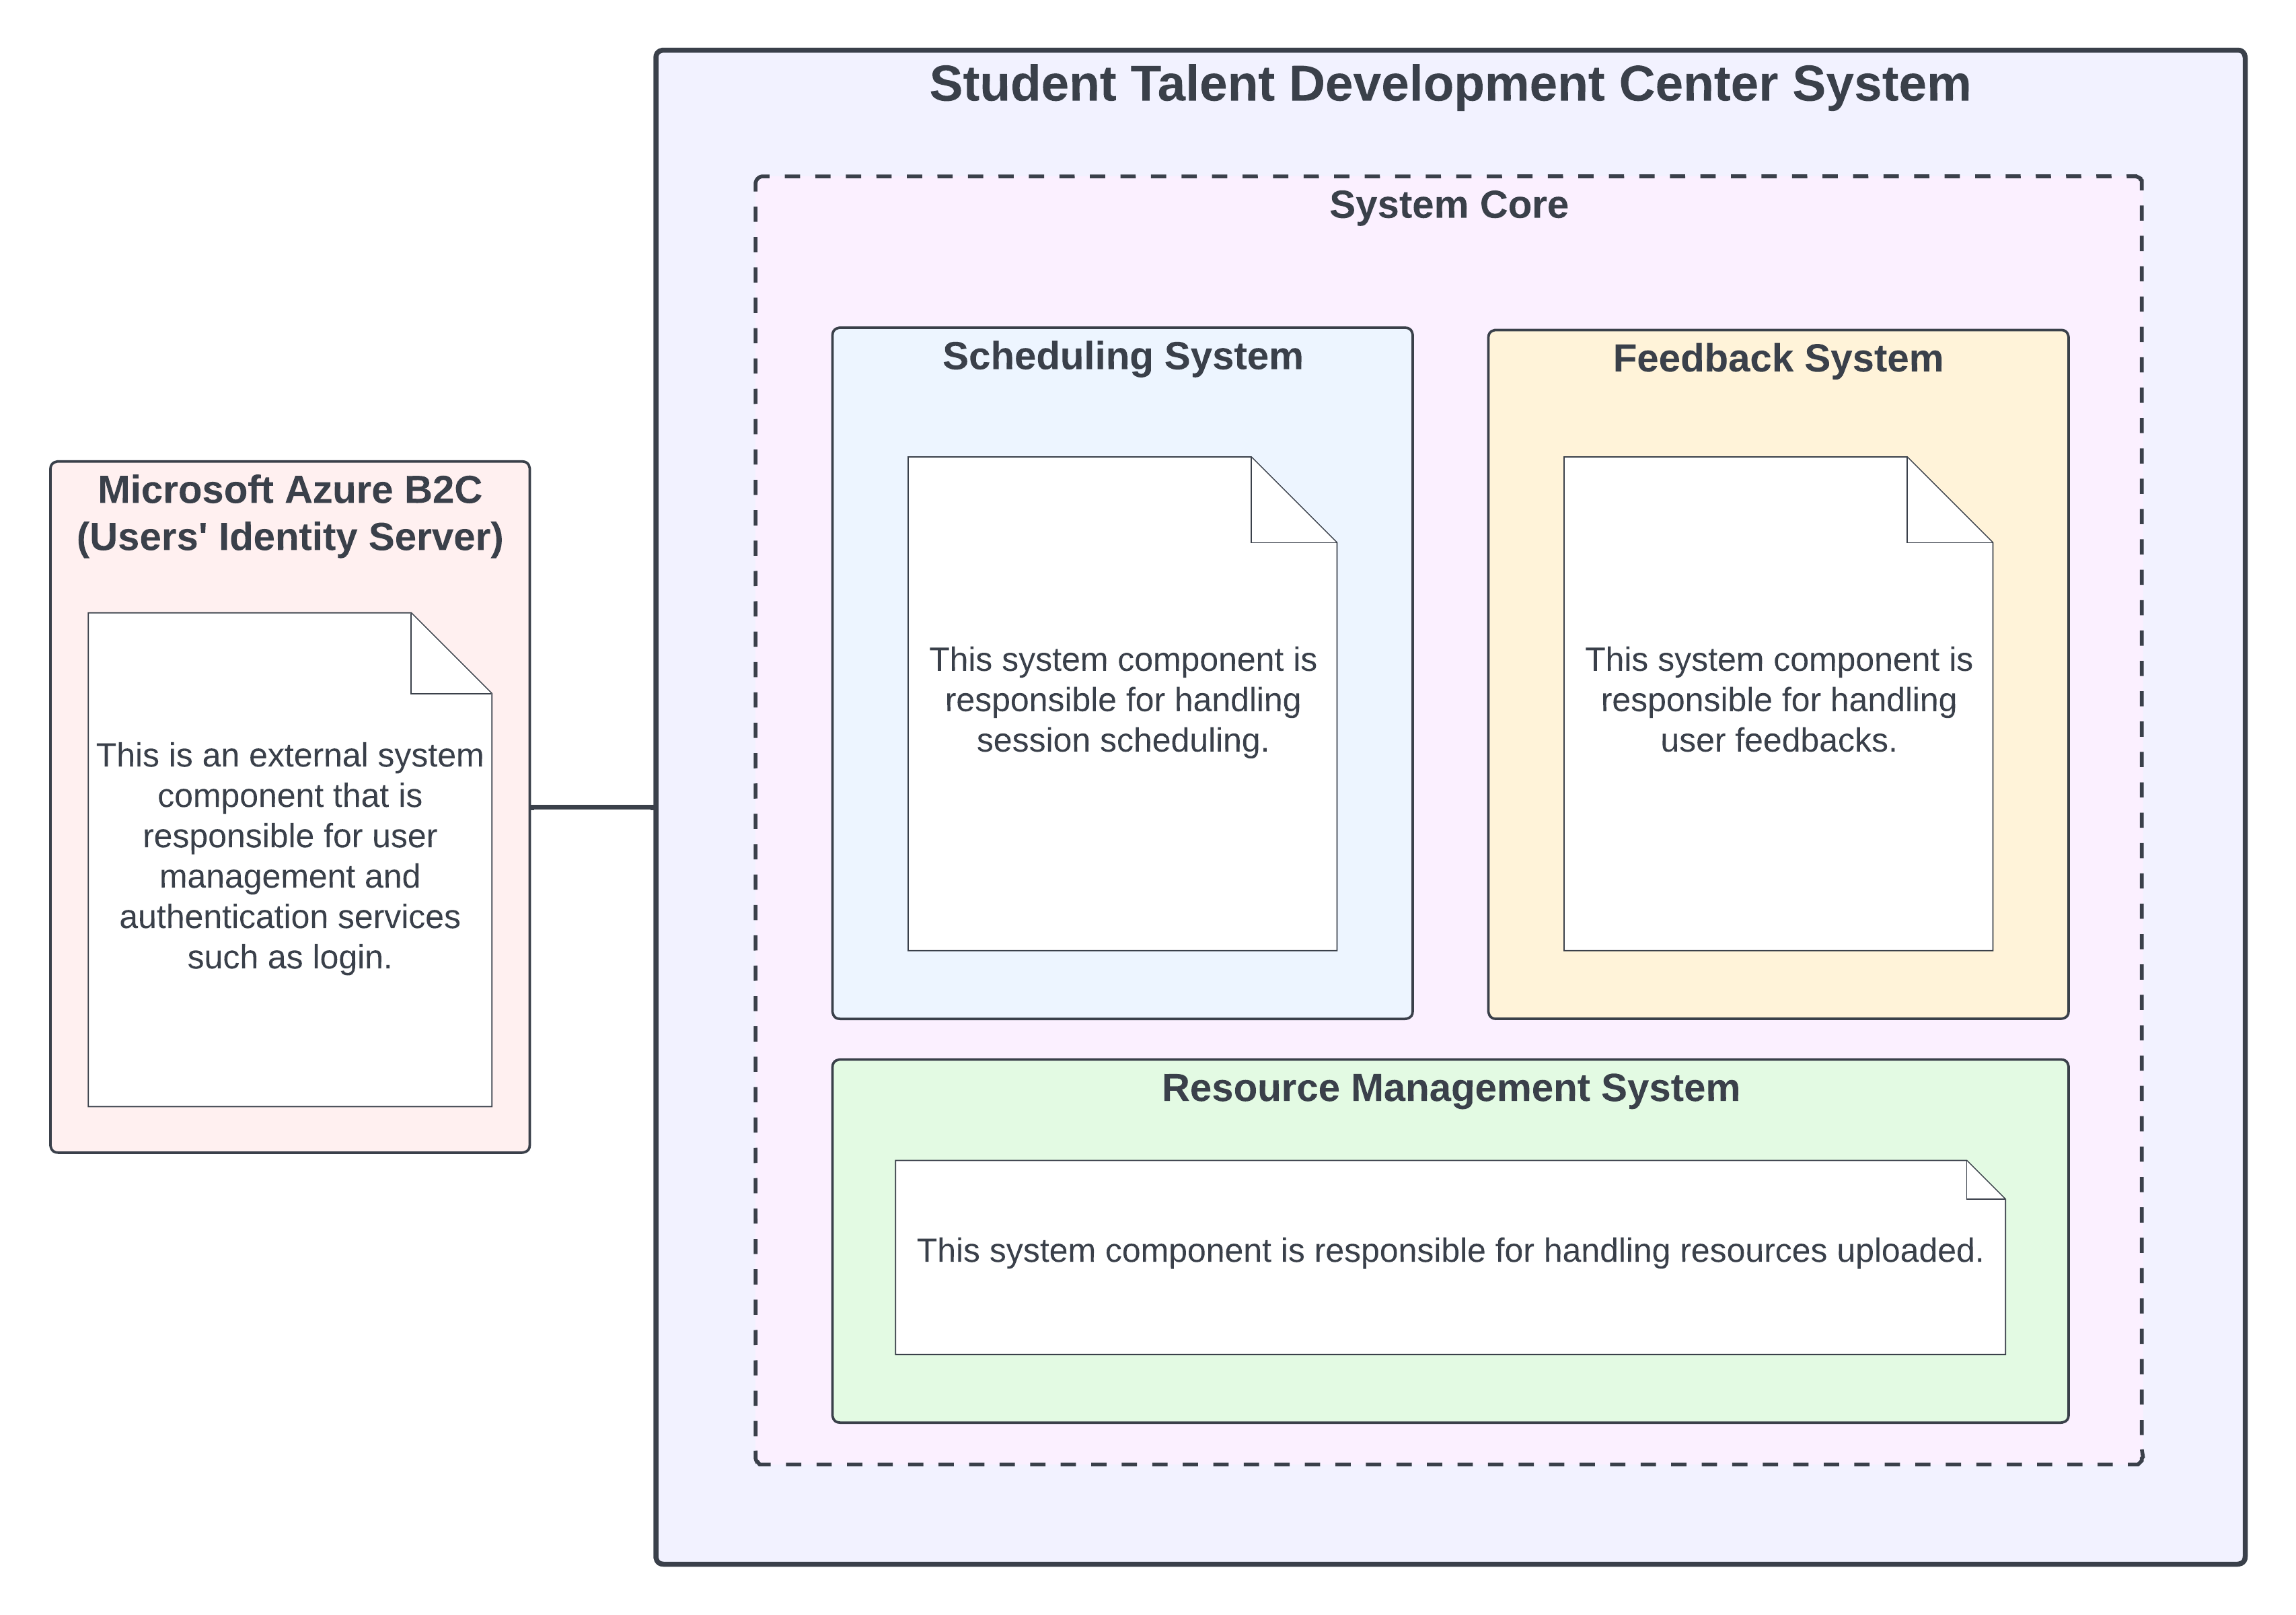
\includegraphics[width=150mm,scale=1]{figures/analysis_and_design/analysis/1. Conceptual System Overview.png}}
    \caption{Use case model - conceptual system overview}
    \label{ConceptualSystemOverview}
\end{figure}

\begin{figure}[H]
    \centerline{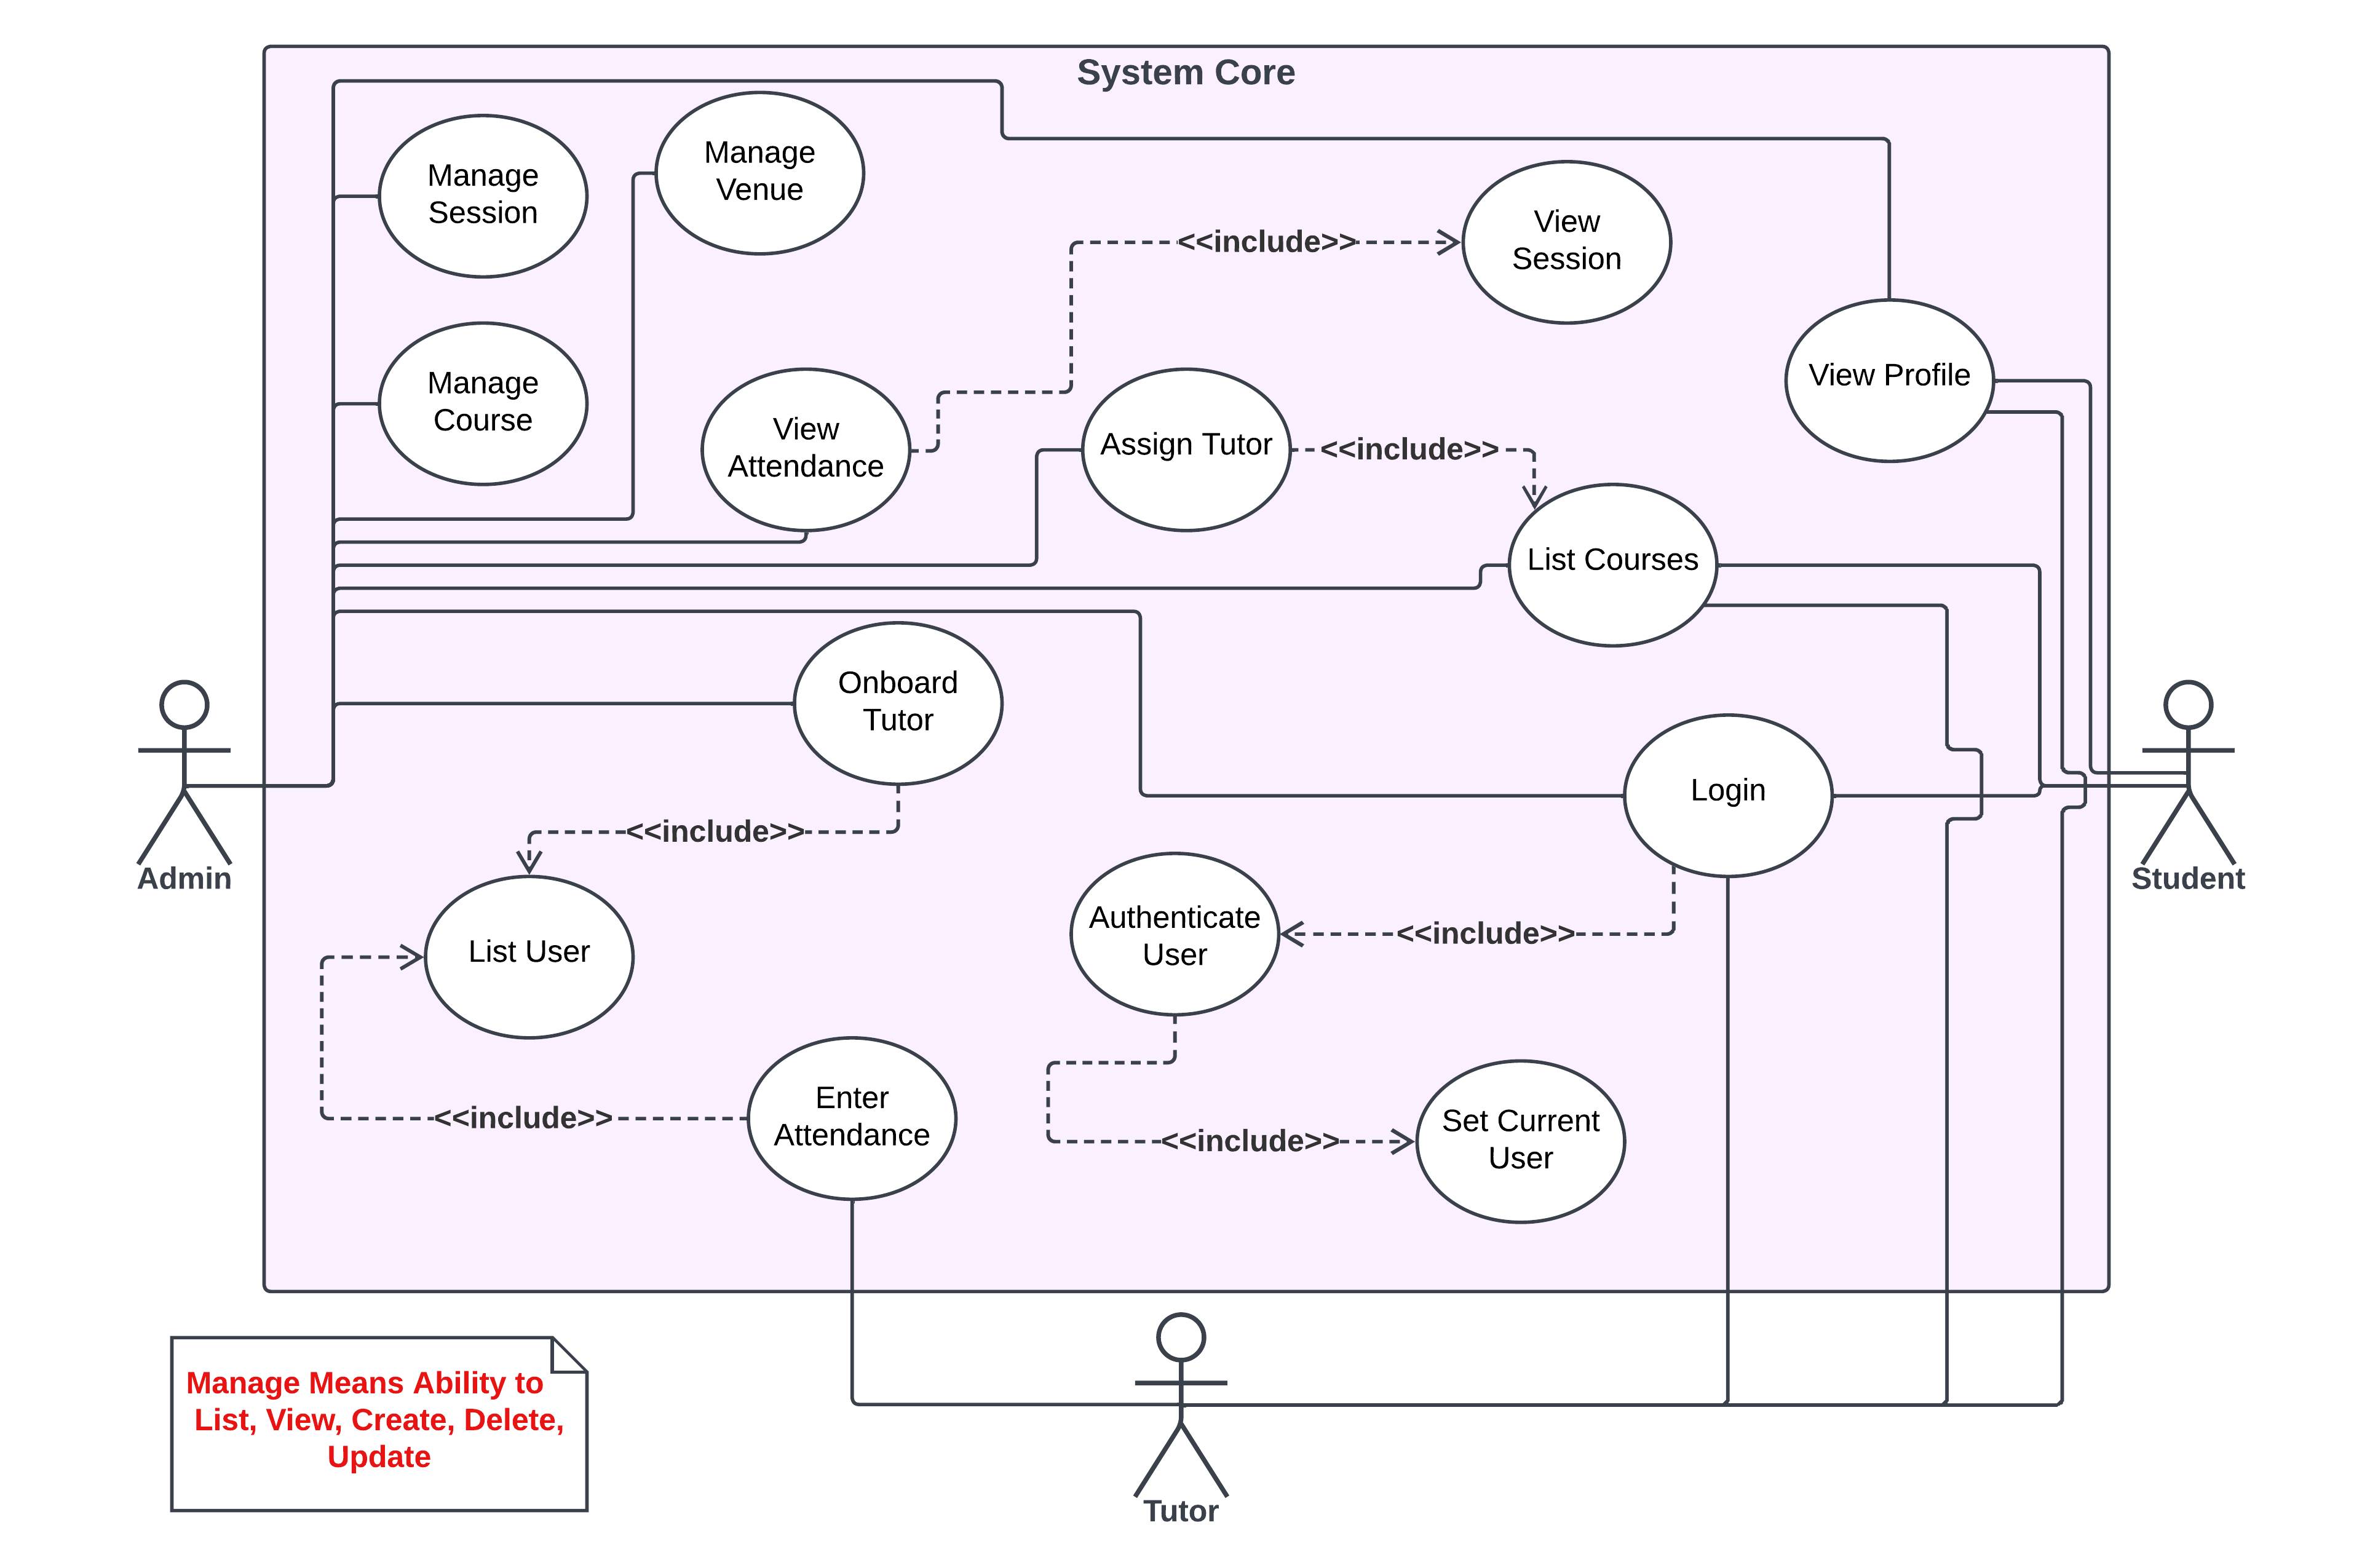
\includegraphics[width=150mm,scale=1]{figures/analysis_and_design/analysis/2. System Core.png}}
    \caption{Use case model - system core}
    \label{SystemCore}
\end{figure}

\begin{figure}[H]
    \centerline{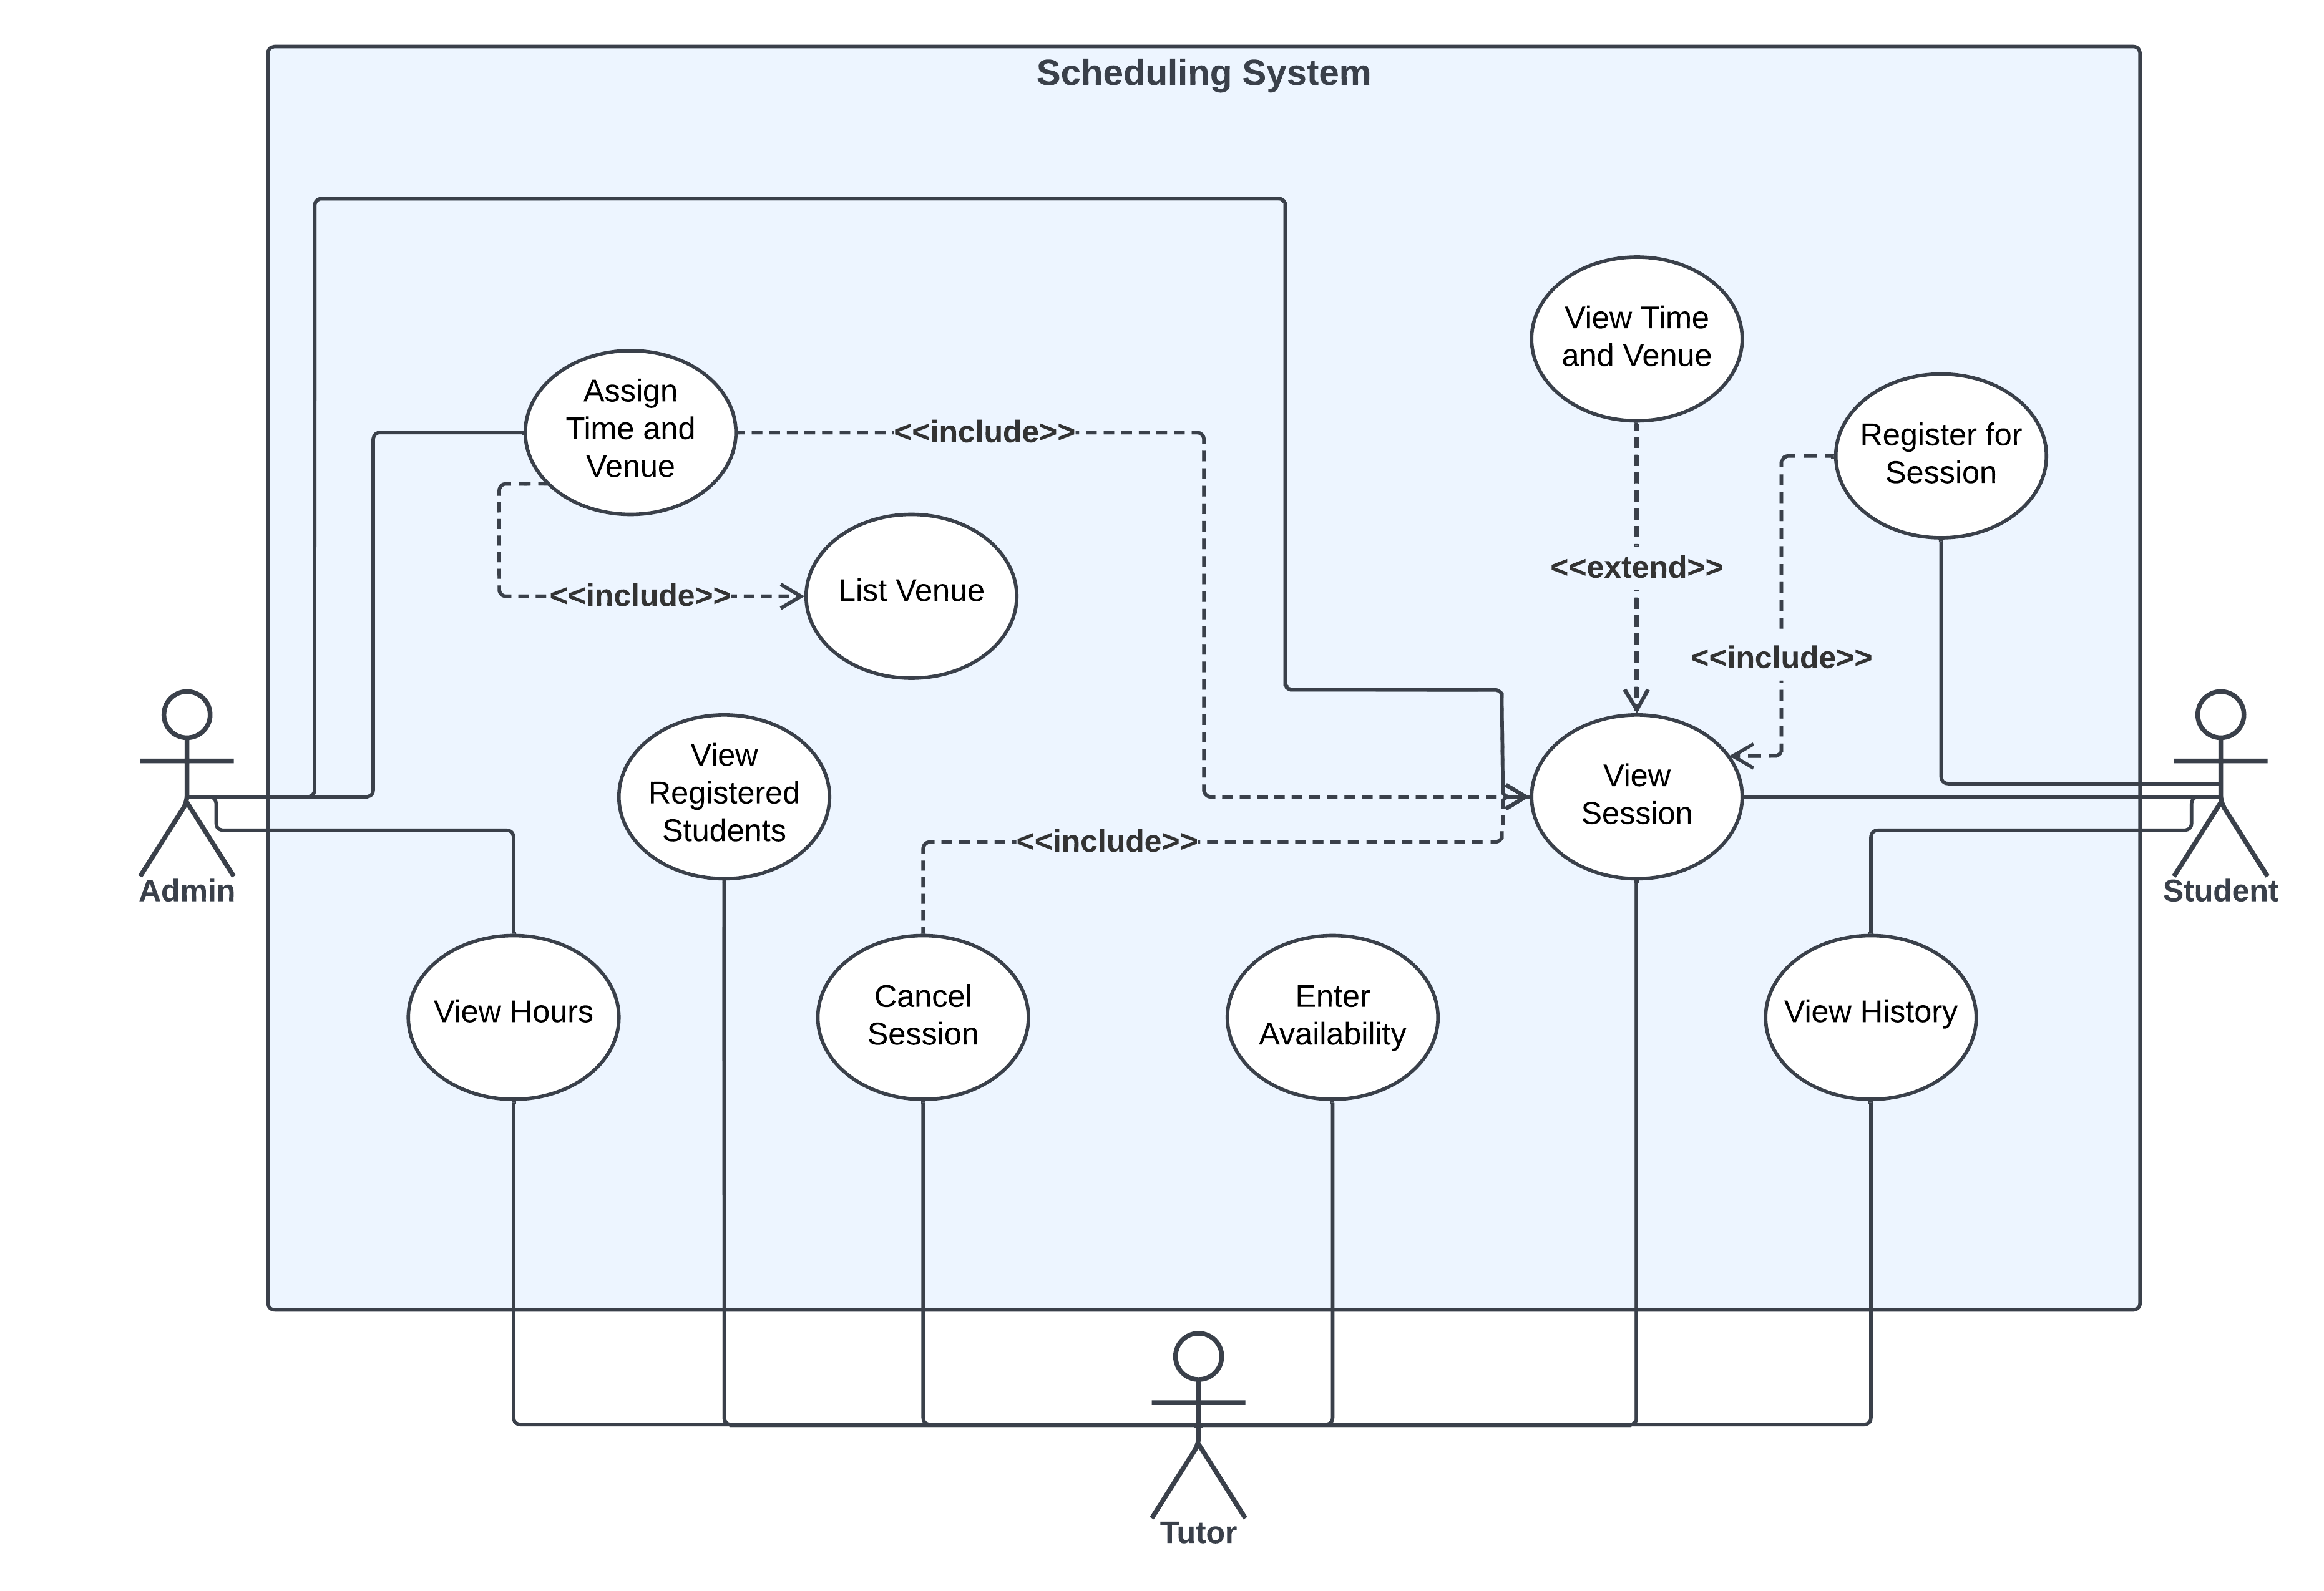
\includegraphics[width=150mm,scale=1]{figures/analysis_and_design/analysis/3. Scheduling System.png}}
    \caption{Use case model - scheduling system}
    \label{SchedulingSystem}
\end{figure}

\begin{figure}[H]
    \centerline{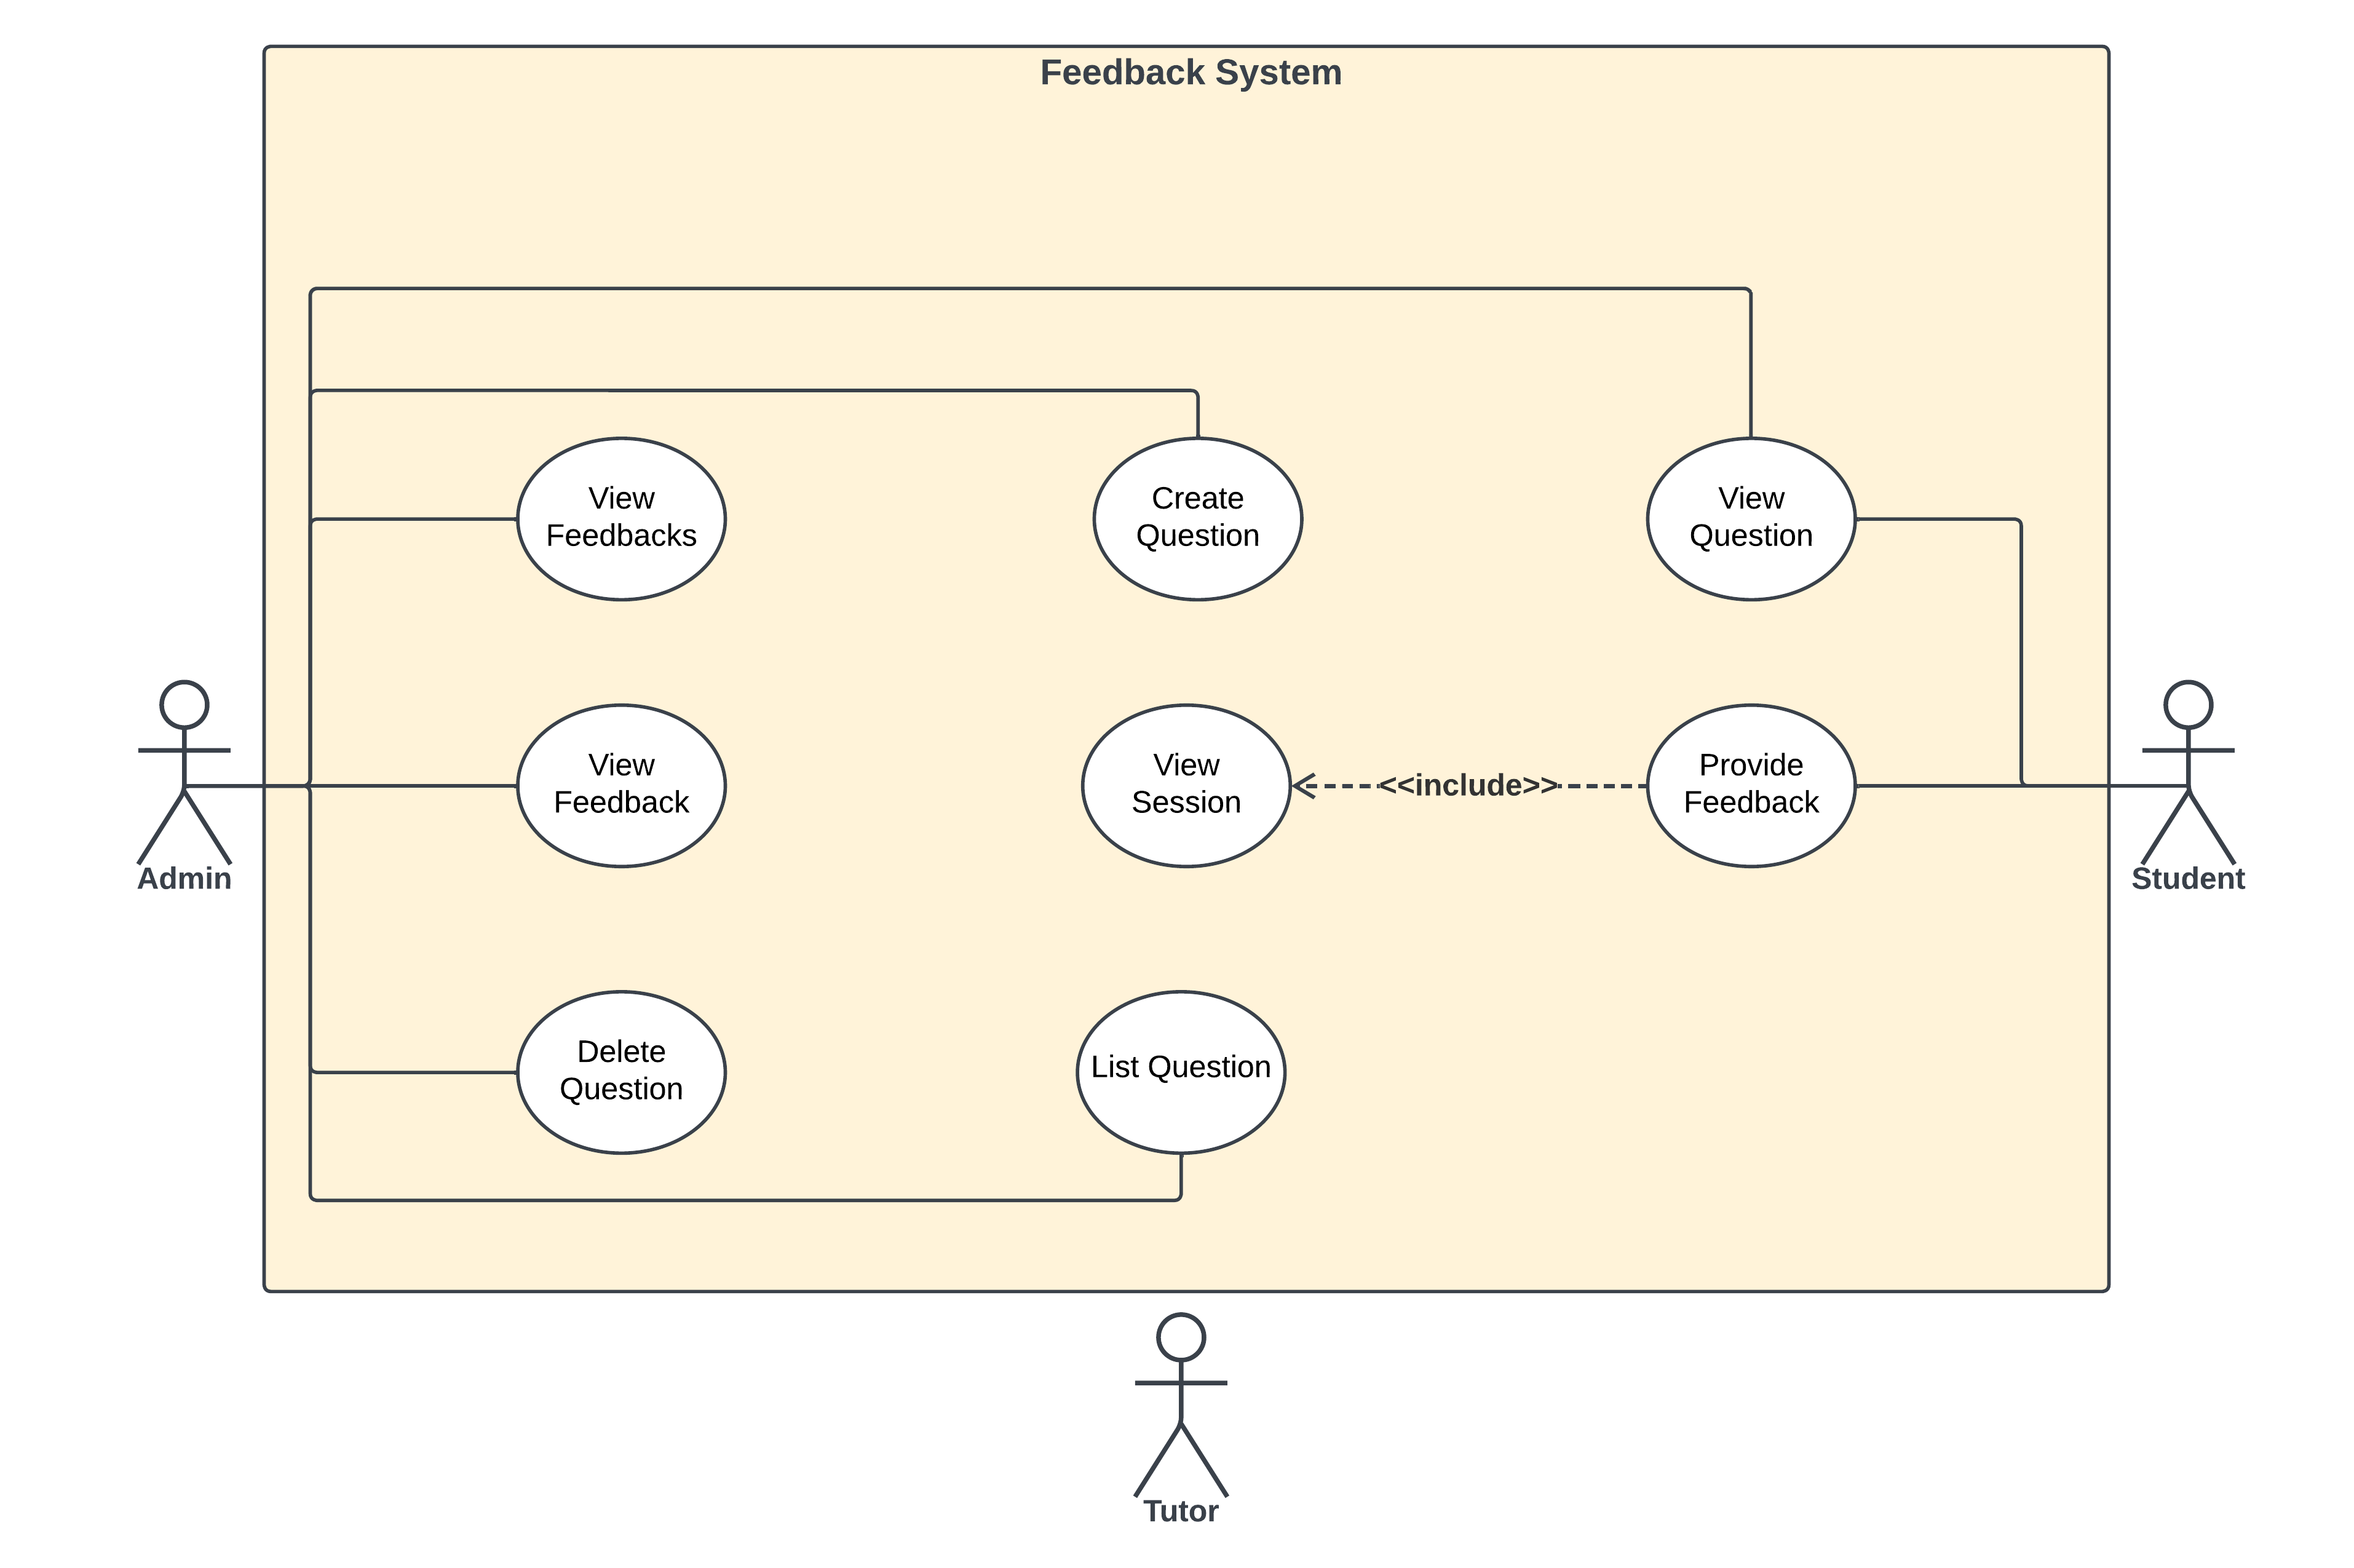
\includegraphics[width=150mm,scale=1]{figures/analysis_and_design/analysis/4. Feedback System.png}}
    \caption{Use case model - feedback system}
    \label{FeedbackSystem}
\end{figure}

\begin{figure}[H]
    \centerline{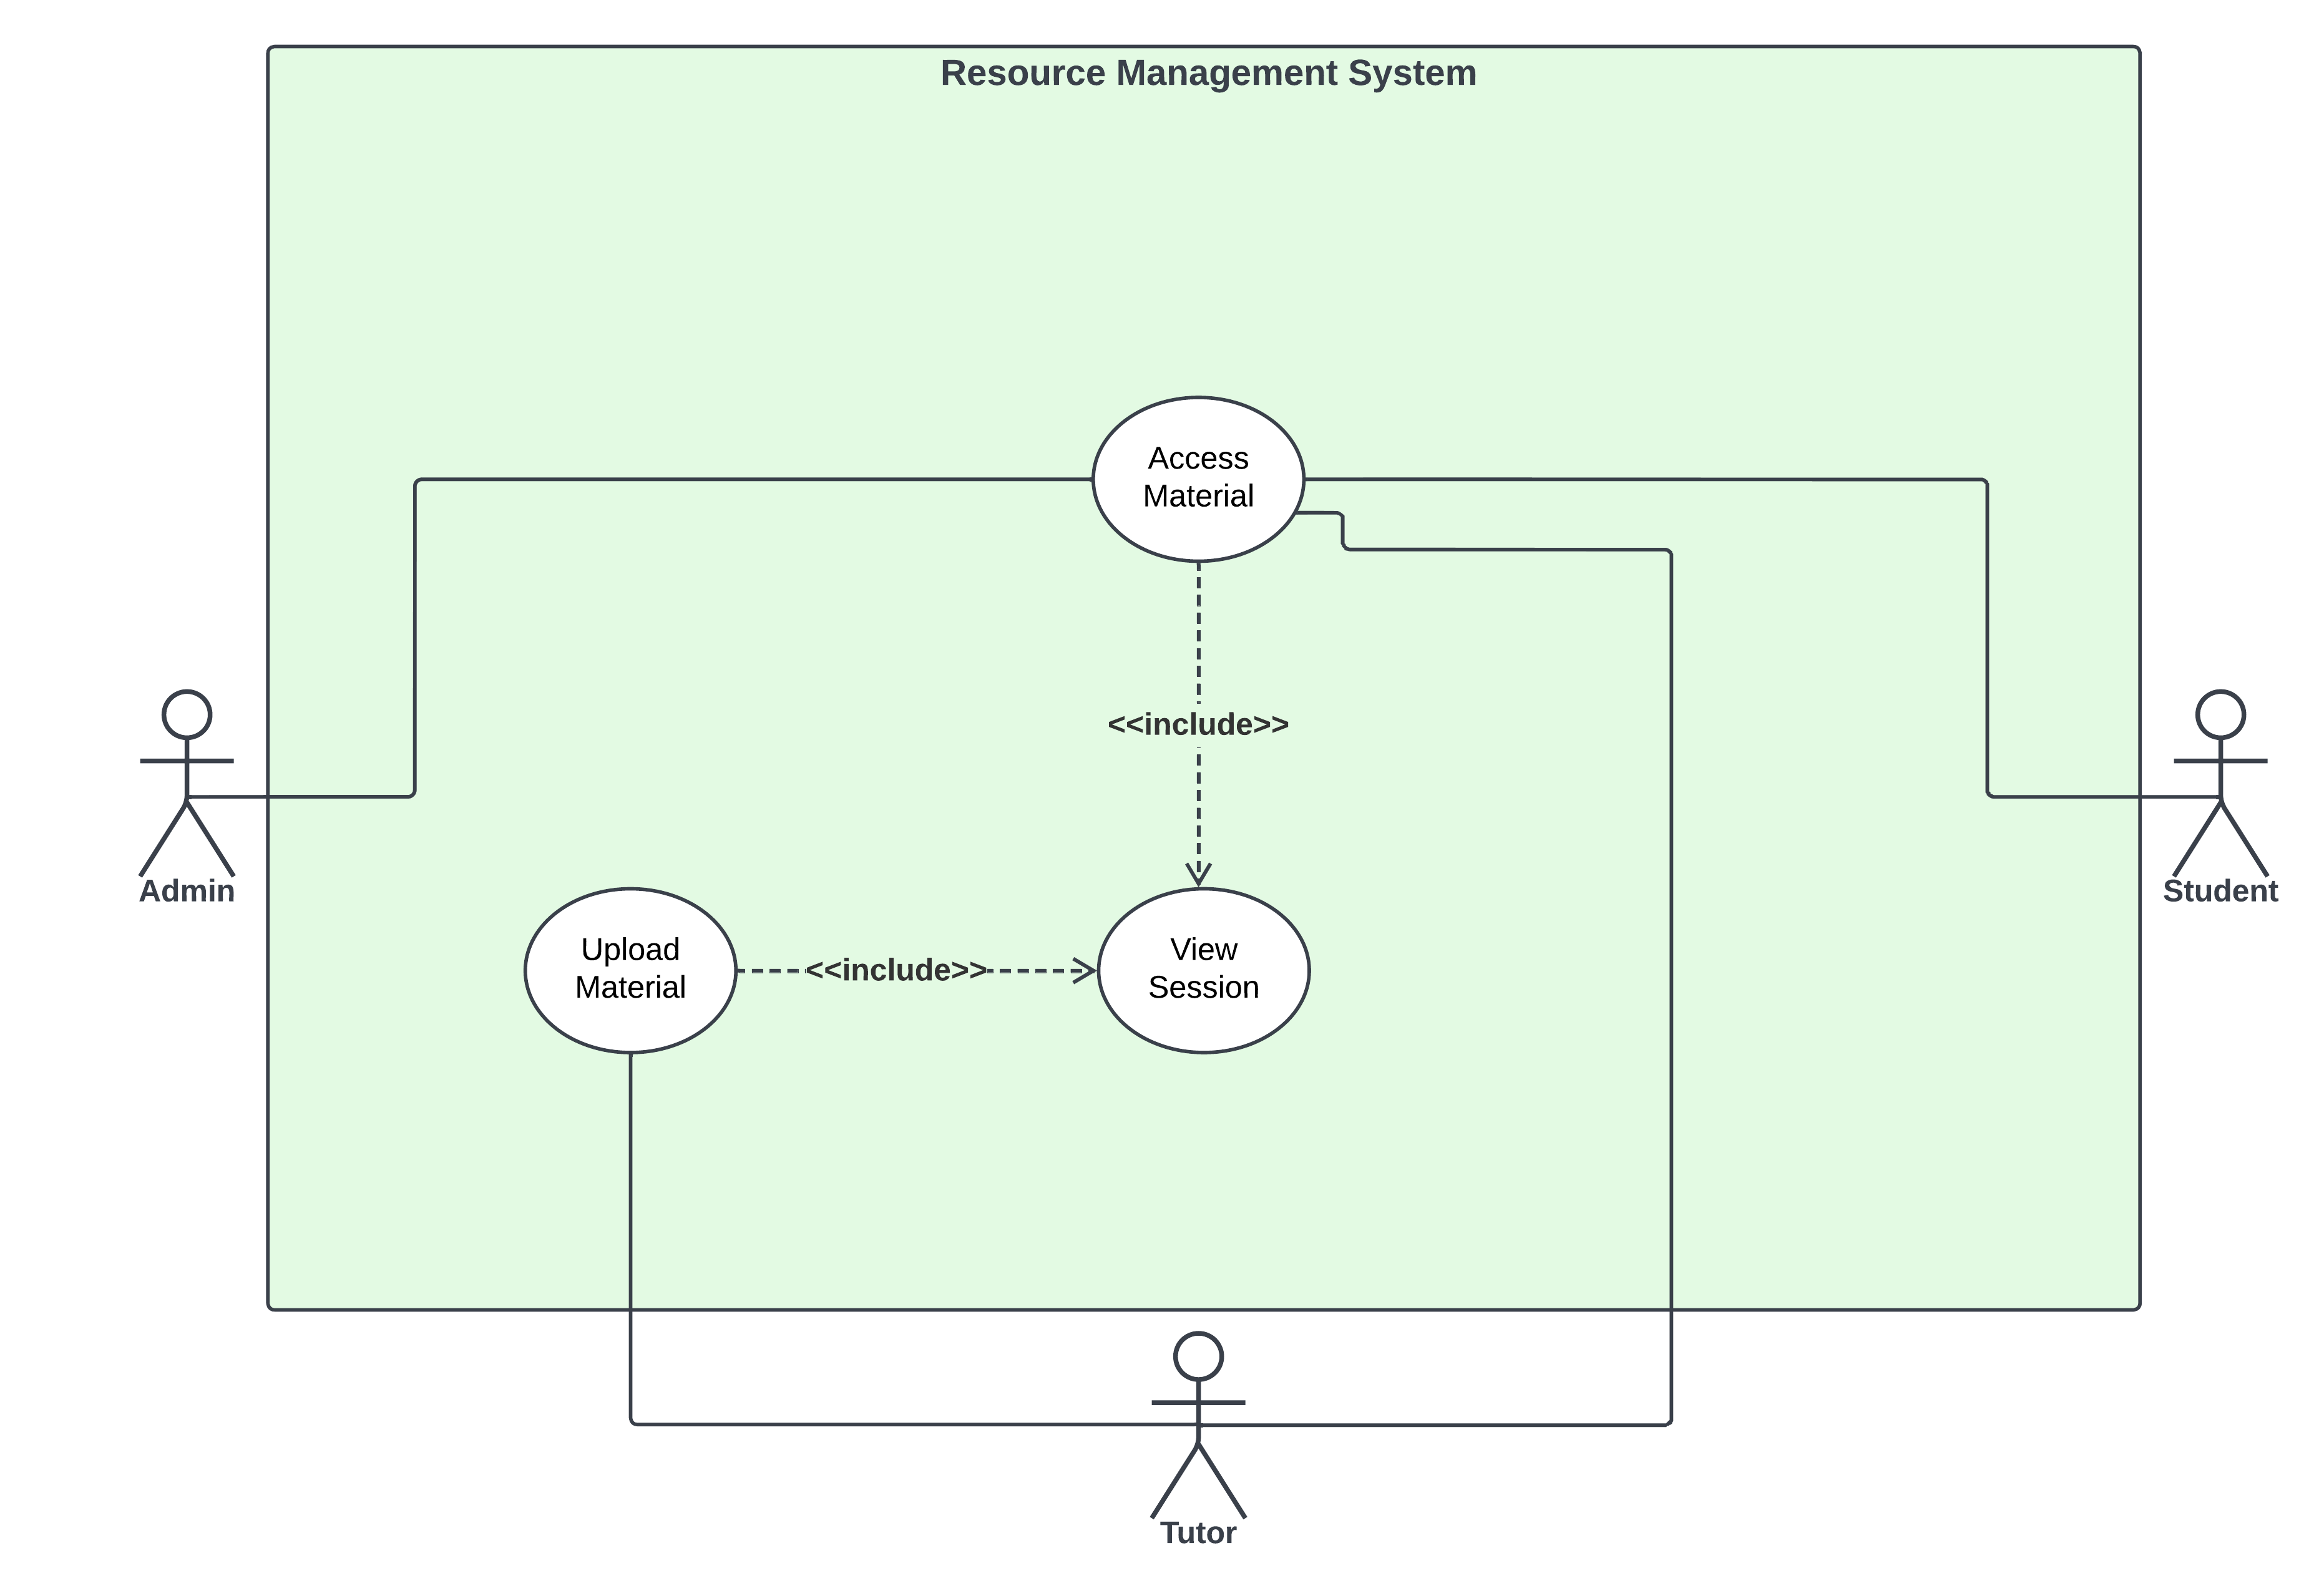
\includegraphics[width=150mm,scale=1]{figures/analysis_and_design/analysis/5. Resource Management System.png}}
    \caption{Use case model - resource management system}
    \label{ResourceManagementSystem}
\end{figure}

\clearpage
\newendline\textbf{Use Case Tabular Form}\newendline
The use case tabular form is a detailed version of the above UML Use Cases. Each use case is explained in detail with specified steps, preconditions, post conditions, input, trigger, and so on. Below here the table entries are explain and one example of these use cases are provided, however the rest can be accessed in the Appendix {\pageref{Appendix 1}}.\\

\renewcommand{\arraystretch}{1.6}
\begin{table}[H]
\centering
\caption{Use case tabular form -- fields' description }
\arrayrulecolor{black}
\begin{tabular}{!{\color{black}\vrule}l!{\color{black}\vrule}l!{\color{black}\vrule}} 
\hline
\rowcolor[rgb]{0.835,0.863,0.894} \textbf{Use Case Field}    & \textbf{Description}                                          \\ 
\hline
{\cellcolor[rgb]{0.949,0.949,0.949}}\textbf{Use Case ID}     & Unique
  ID associated with the use case.                     \\ 
\hline
{\cellcolor[rgb]{0.949,0.949,0.949}}\textbf{Version}         & Last
  updated version.                                       \\ 
\hline
{\cellcolor[rgb]{0.949,0.949,0.949}}\textbf{Last Updated}    & Date of
  the last modification to the use case.              \\ 
\hline
{\cellcolor[rgb]{0.949,0.949,0.949}}\textbf{Name}            & Name of
  the use case.                                       \\ 
\hline
{\cellcolor[rgb]{0.949,0.949,0.949}}\textbf{Traceability to} & Related
  documents that are associated with the use case.    \\ 
\hline
{\cellcolor[rgb]{0.949,0.949,0.949}}\textbf{Actor}           & All
  users who initiate and participate in the use case.     \\ 
\hline
{\cellcolor[rgb]{0.949,0.949,0.949}}\textbf{Preconditions}   & Constraints
  that must be met for the use case to be taken.  \\ 
\hline
{\cellcolor[rgb]{0.949,0.949,0.949}}\textbf{Trigger}         & Event
  that initiates the use case.                          \\ 
\hline
{\cellcolor[rgb]{0.949,0.949,0.949}}\textbf{Input}           & List of
  the data input by the user.                         \\ 
\hline
{\cellcolor[rgb]{0.949,0.949,0.949}}\textbf{Steps}           & Steps
  needed to be taken to reach the use case.             \\ 
\hline
{\cellcolor[rgb]{0.949,0.949,0.949}}\textbf{Postconditions}  & Constraints
  that must be met for the use case to be done.   \\ 
\hline
{\cellcolor[rgb]{0.949,0.949,0.949}}\textbf{Exception Flow}  & Unsuccessful
  ways this use case might end.                  \\ 
\hline
{\cellcolor[rgb]{0.949,0.949,0.949}}\textbf{Expected Output} & The
  expected successful outcome of this use case.           \\
\hline
\end{tabular}
\arrayrulecolor{black}
\end{table}
\end{justify}


\begin{minipage}[trim]{1\textwidth}
    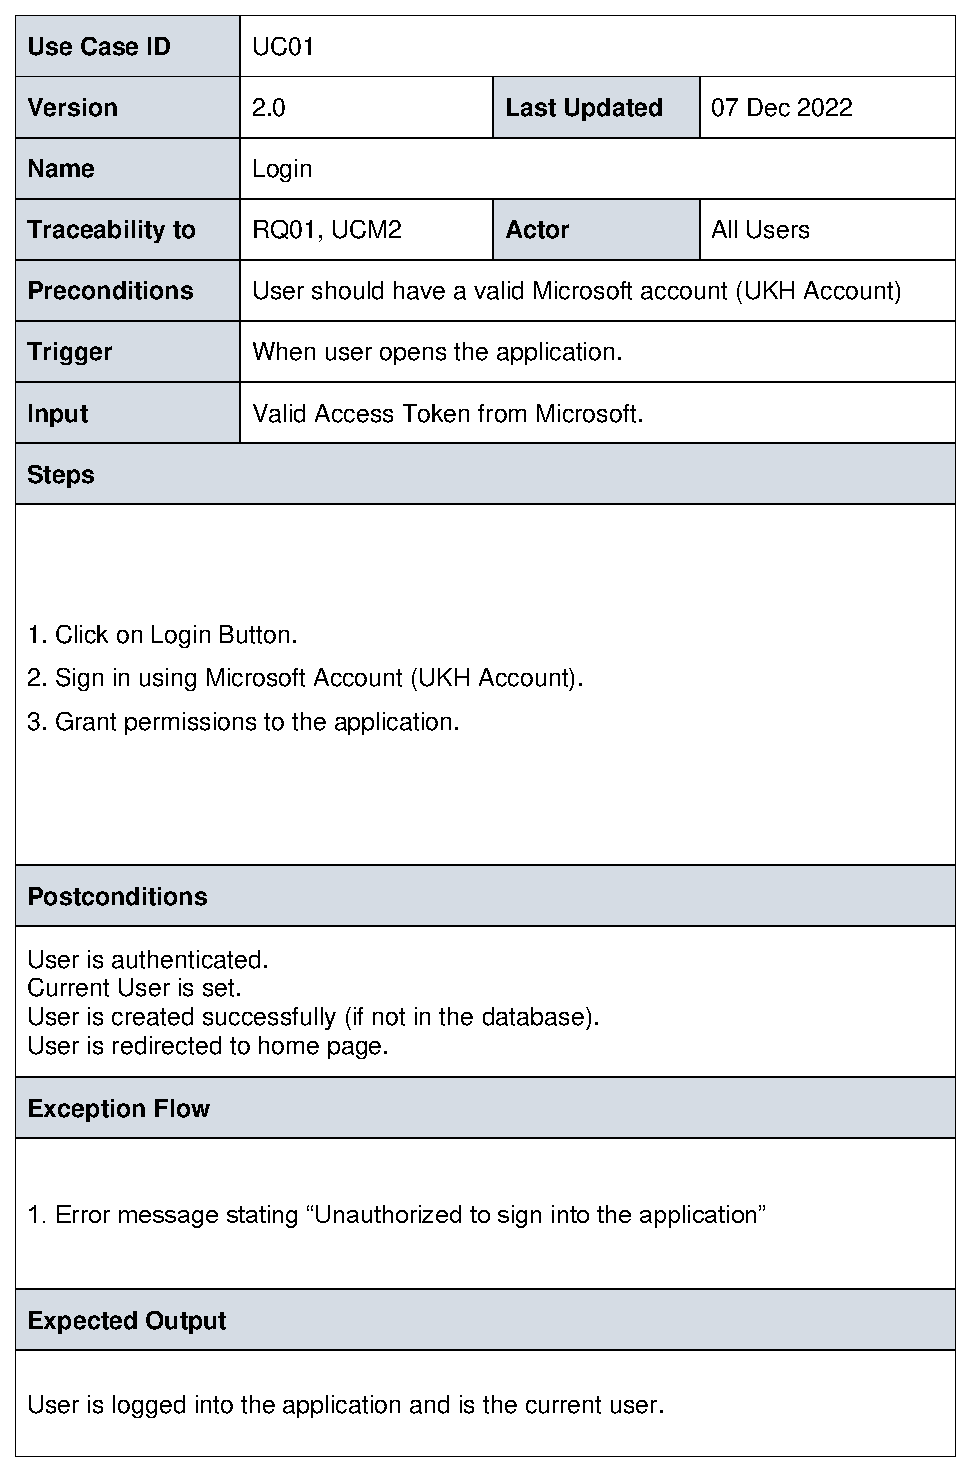
\includegraphics[width=\textwidth]{endpages/appendices/appendix1/table-1.pdf}
\end{minipage}

\clearpage

\newendline\textbf{UML Activity Model}\newendline
The followings are the activity models of one of each component of the system.

\begin{figure}[H]
    \centerline{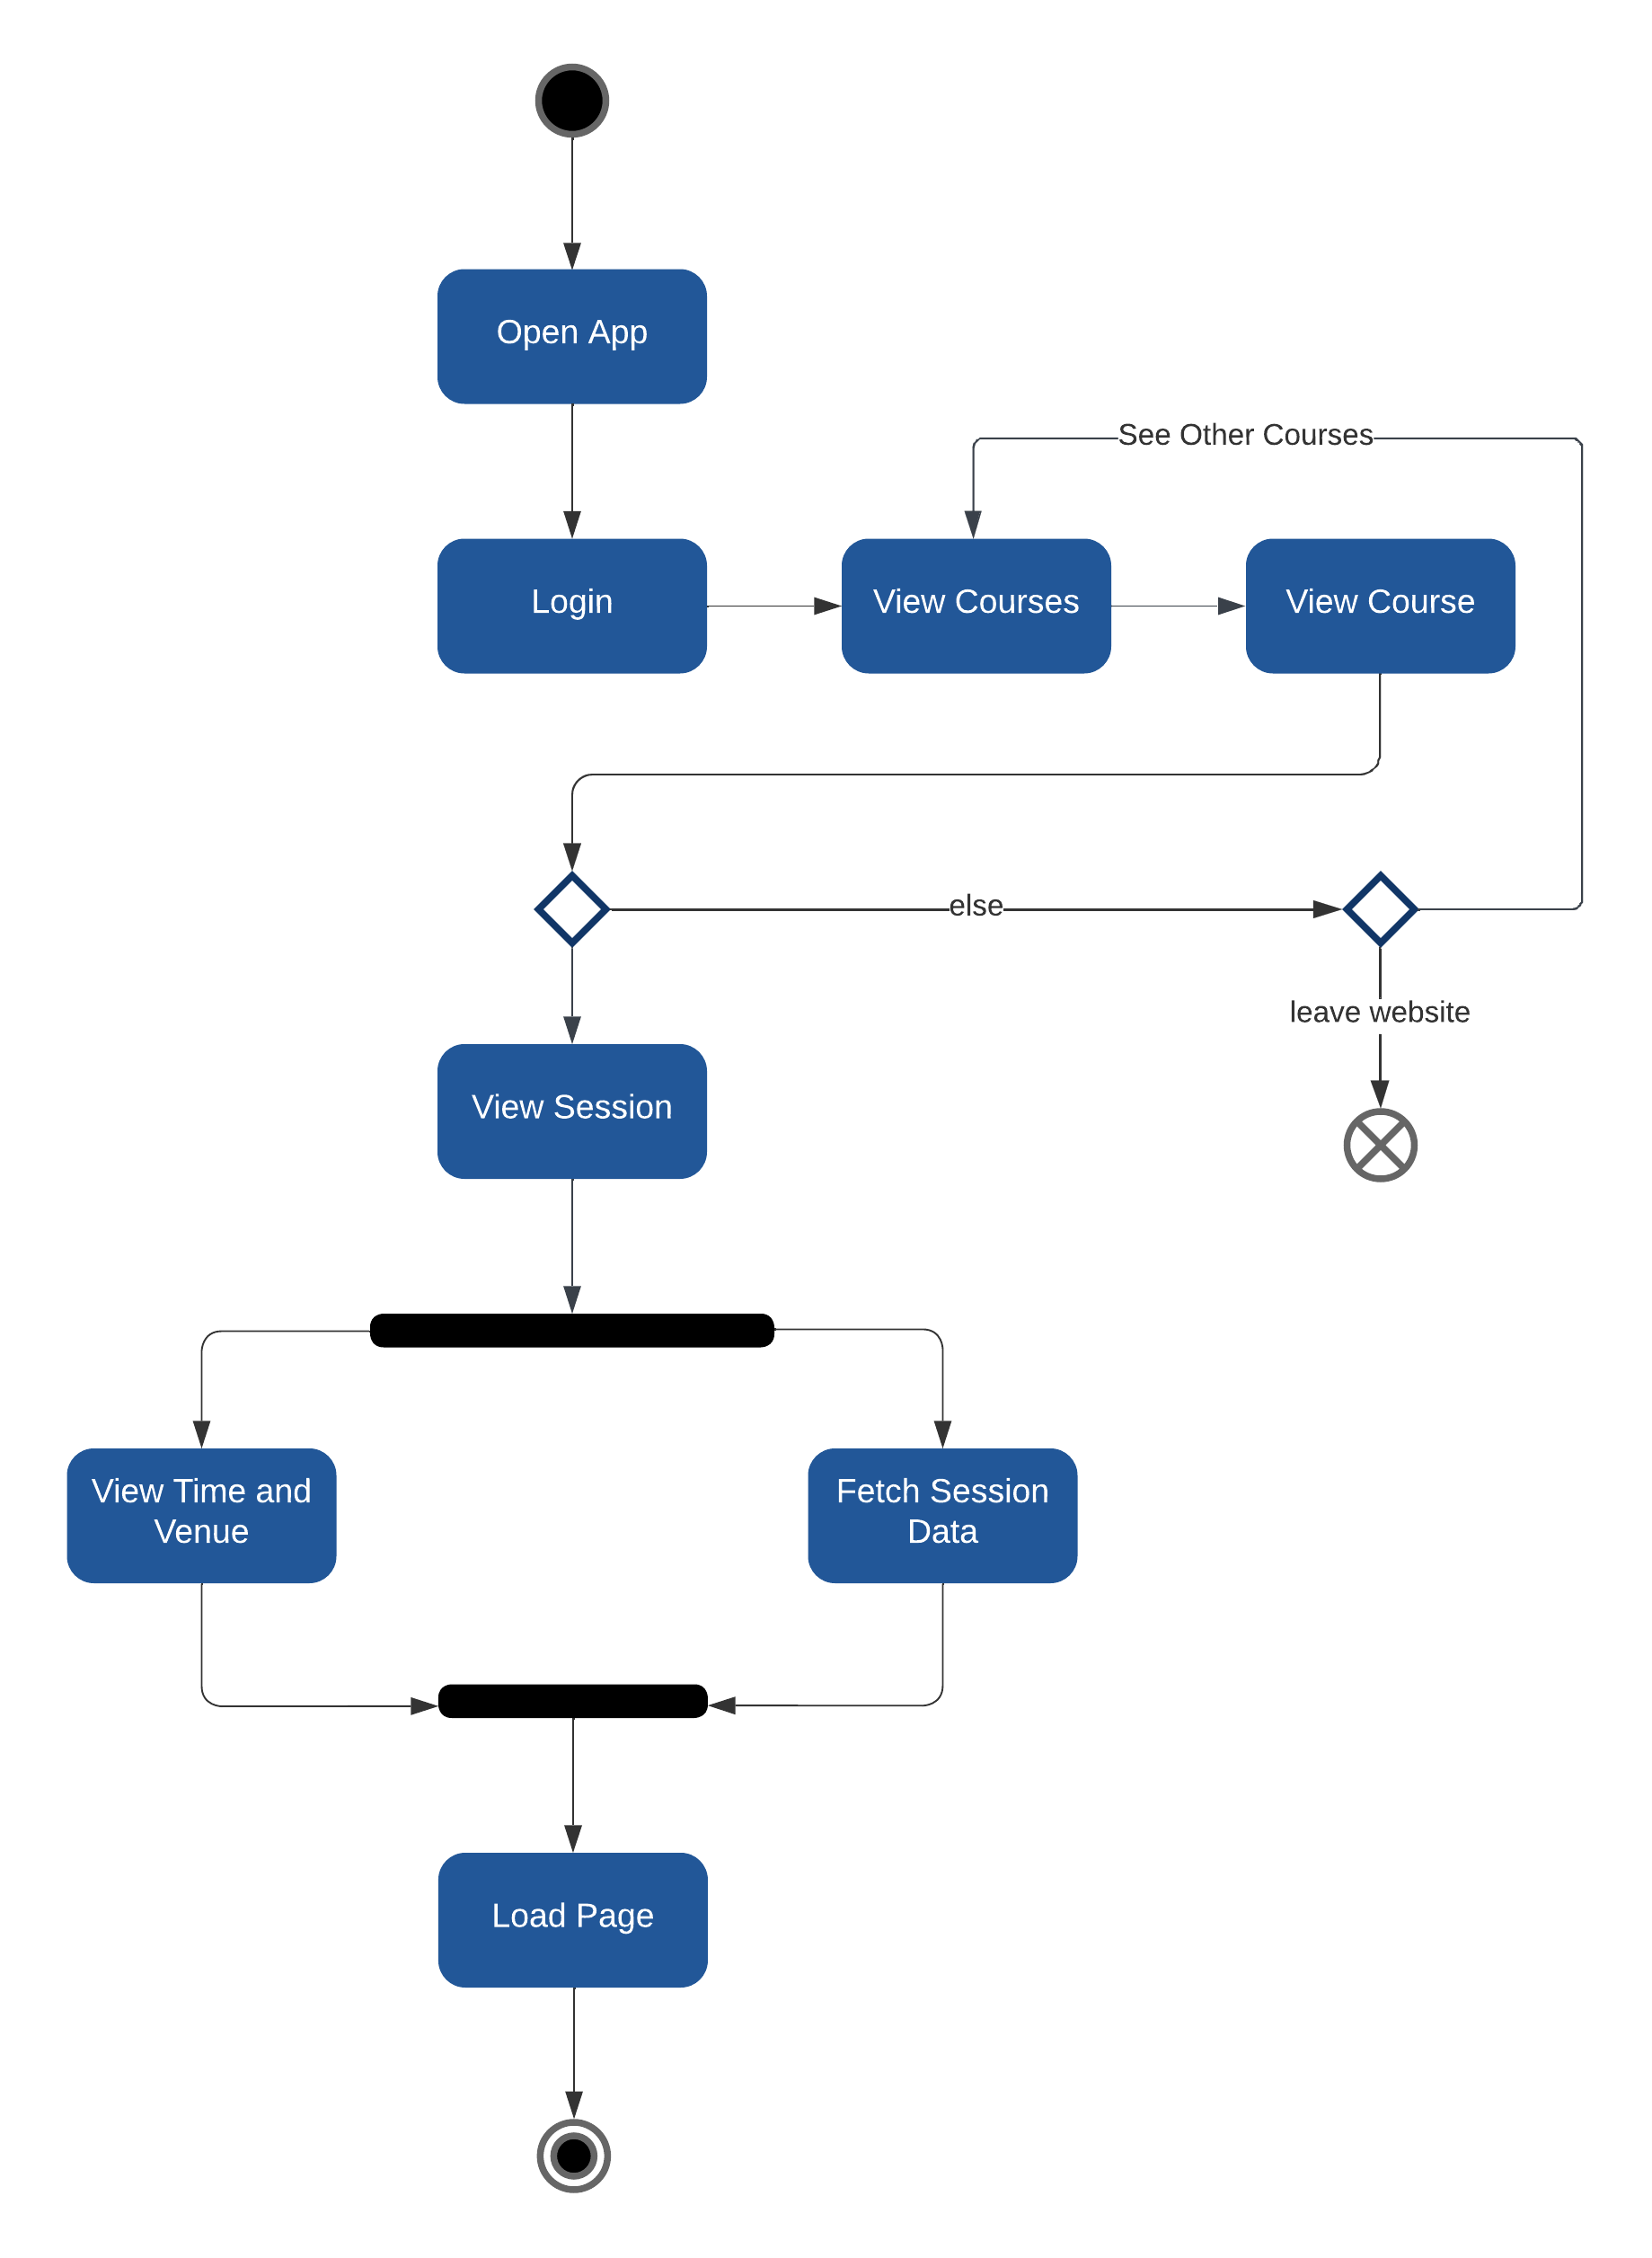
\includegraphics[width=150mm,scale=1]{figures/analysis_and_design/analysis/1. View Session.png}}
    \caption{Activity model - view session}
    \label{viewSession}
\end{figure}

\begin{figure}[H]
    \centerline{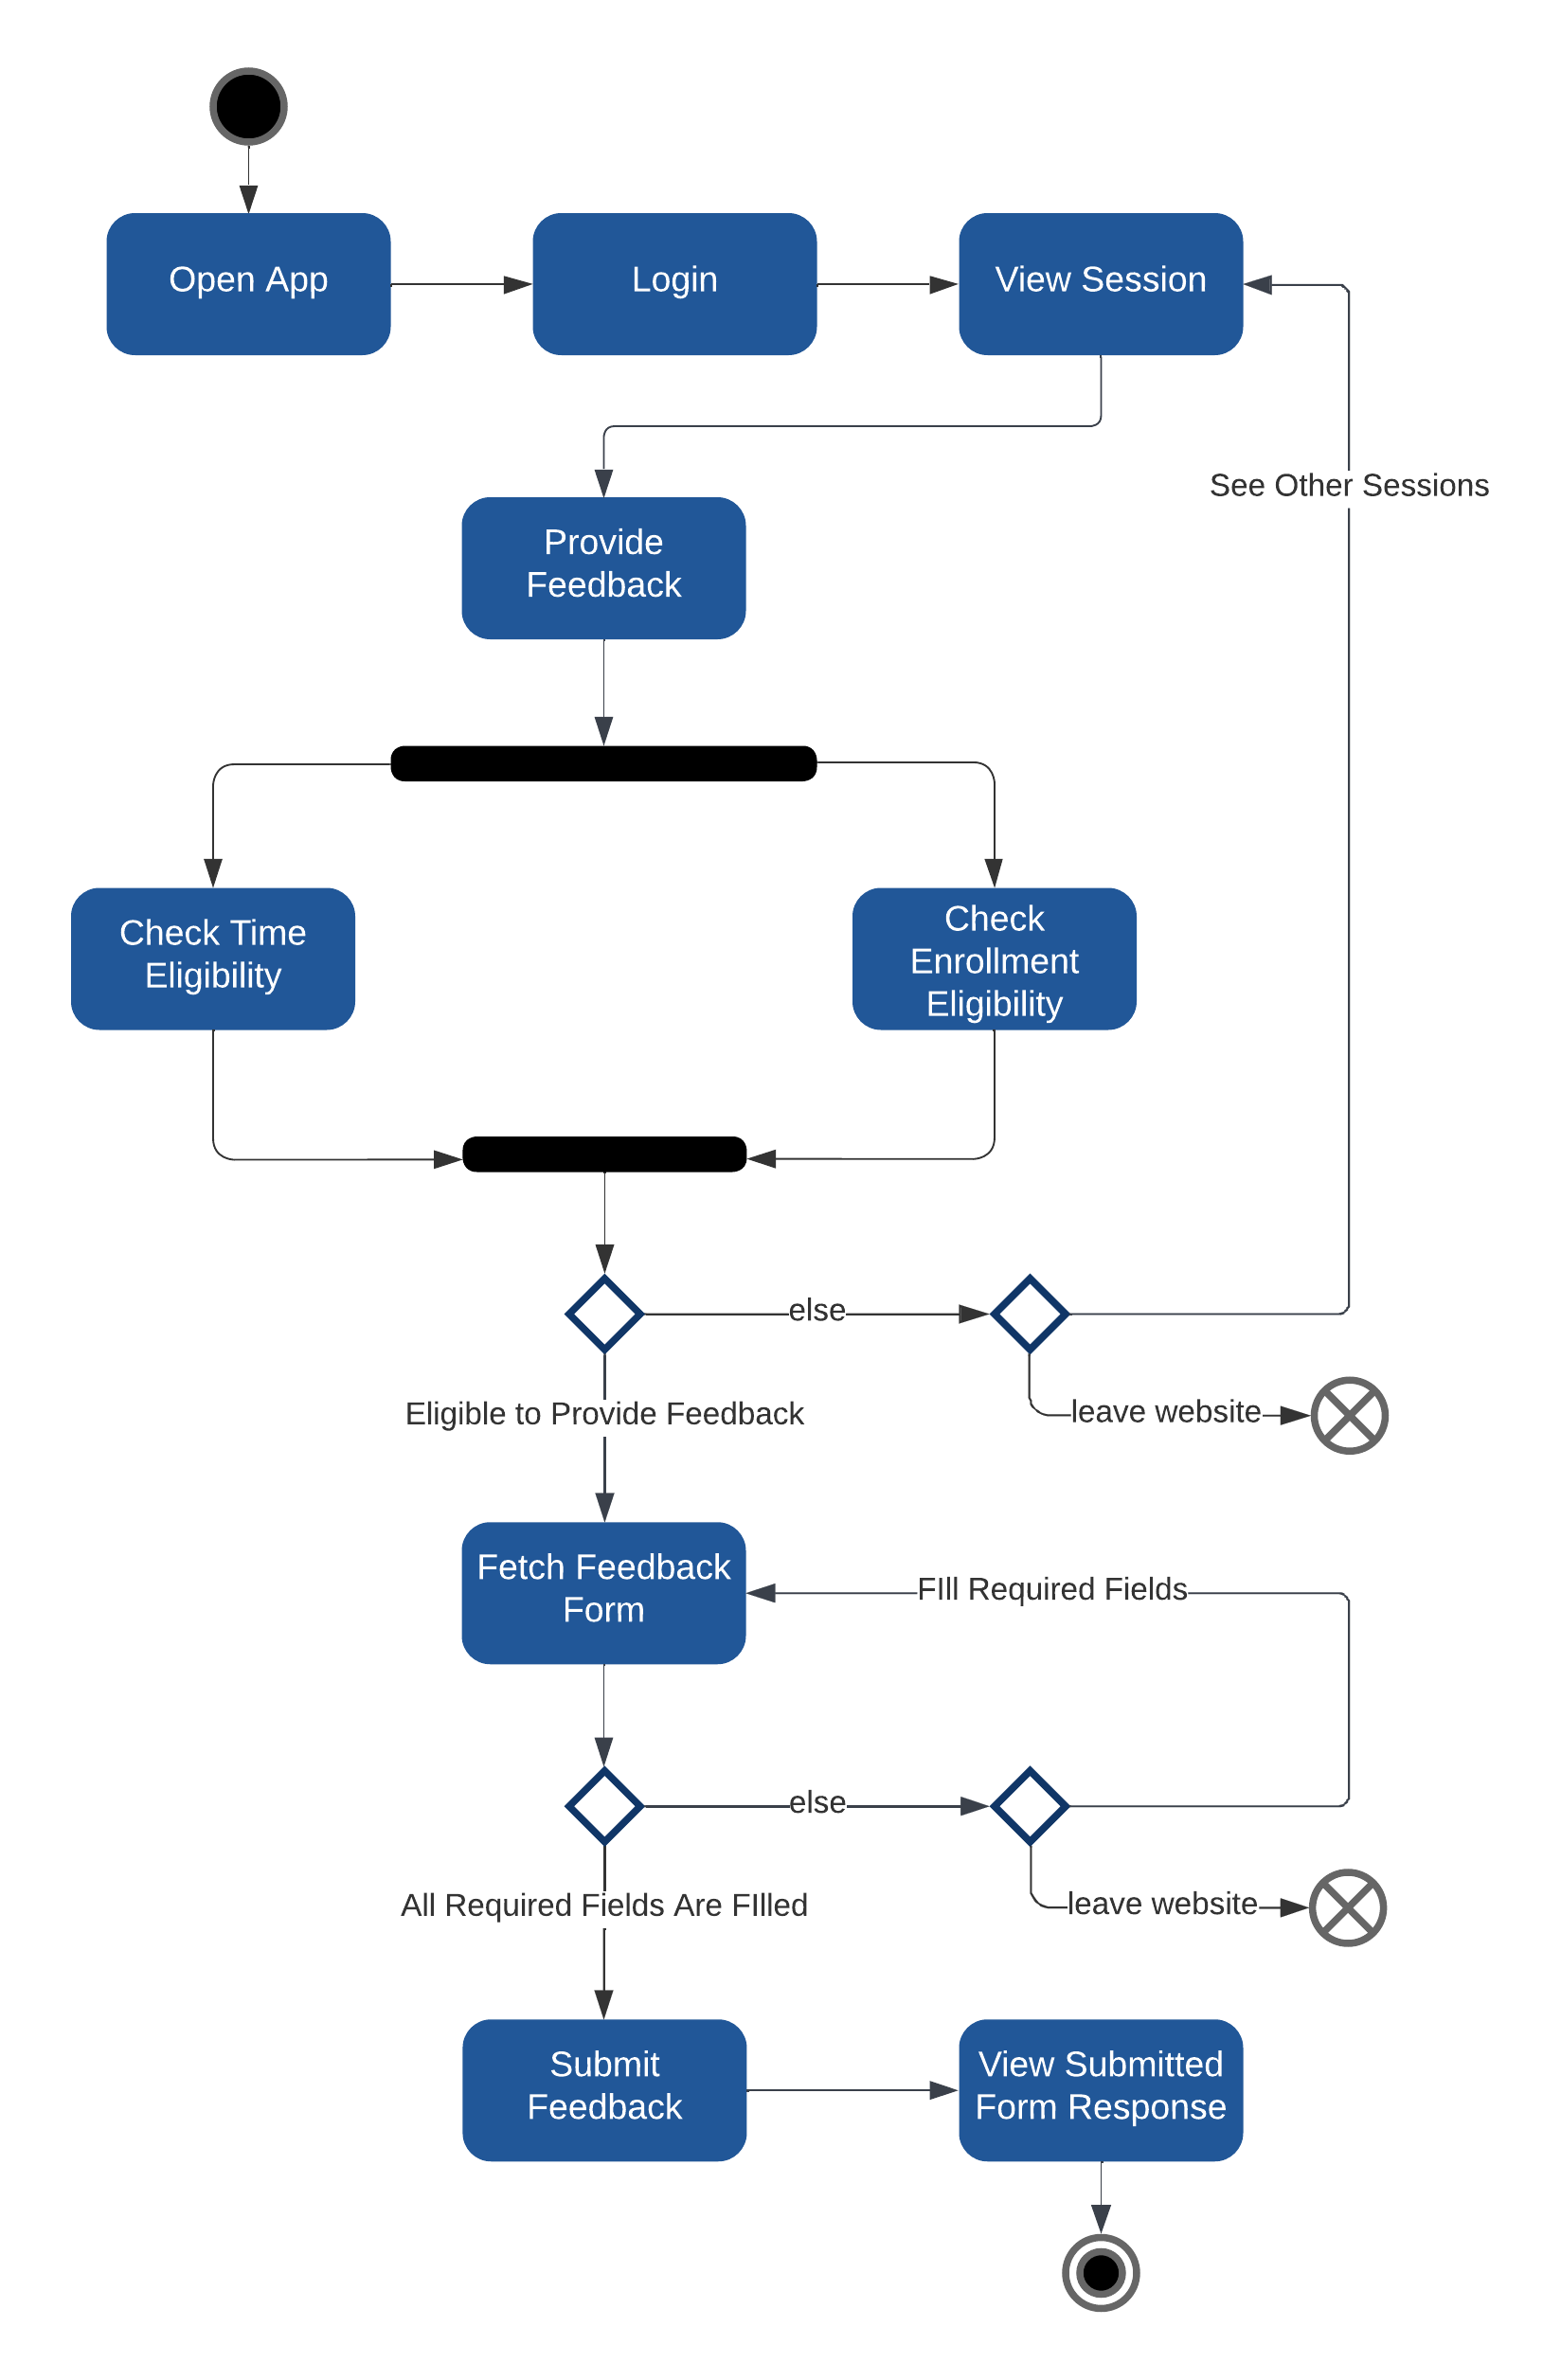
\includegraphics[width=150mm,scale=1]{figures/analysis_and_design/analysis/2. Provide Feedback.png}}
    \caption{Activity model - provide feedback}
    \label{provideFeedback}
\end{figure}

\begin{figure}[H]
    \centerline{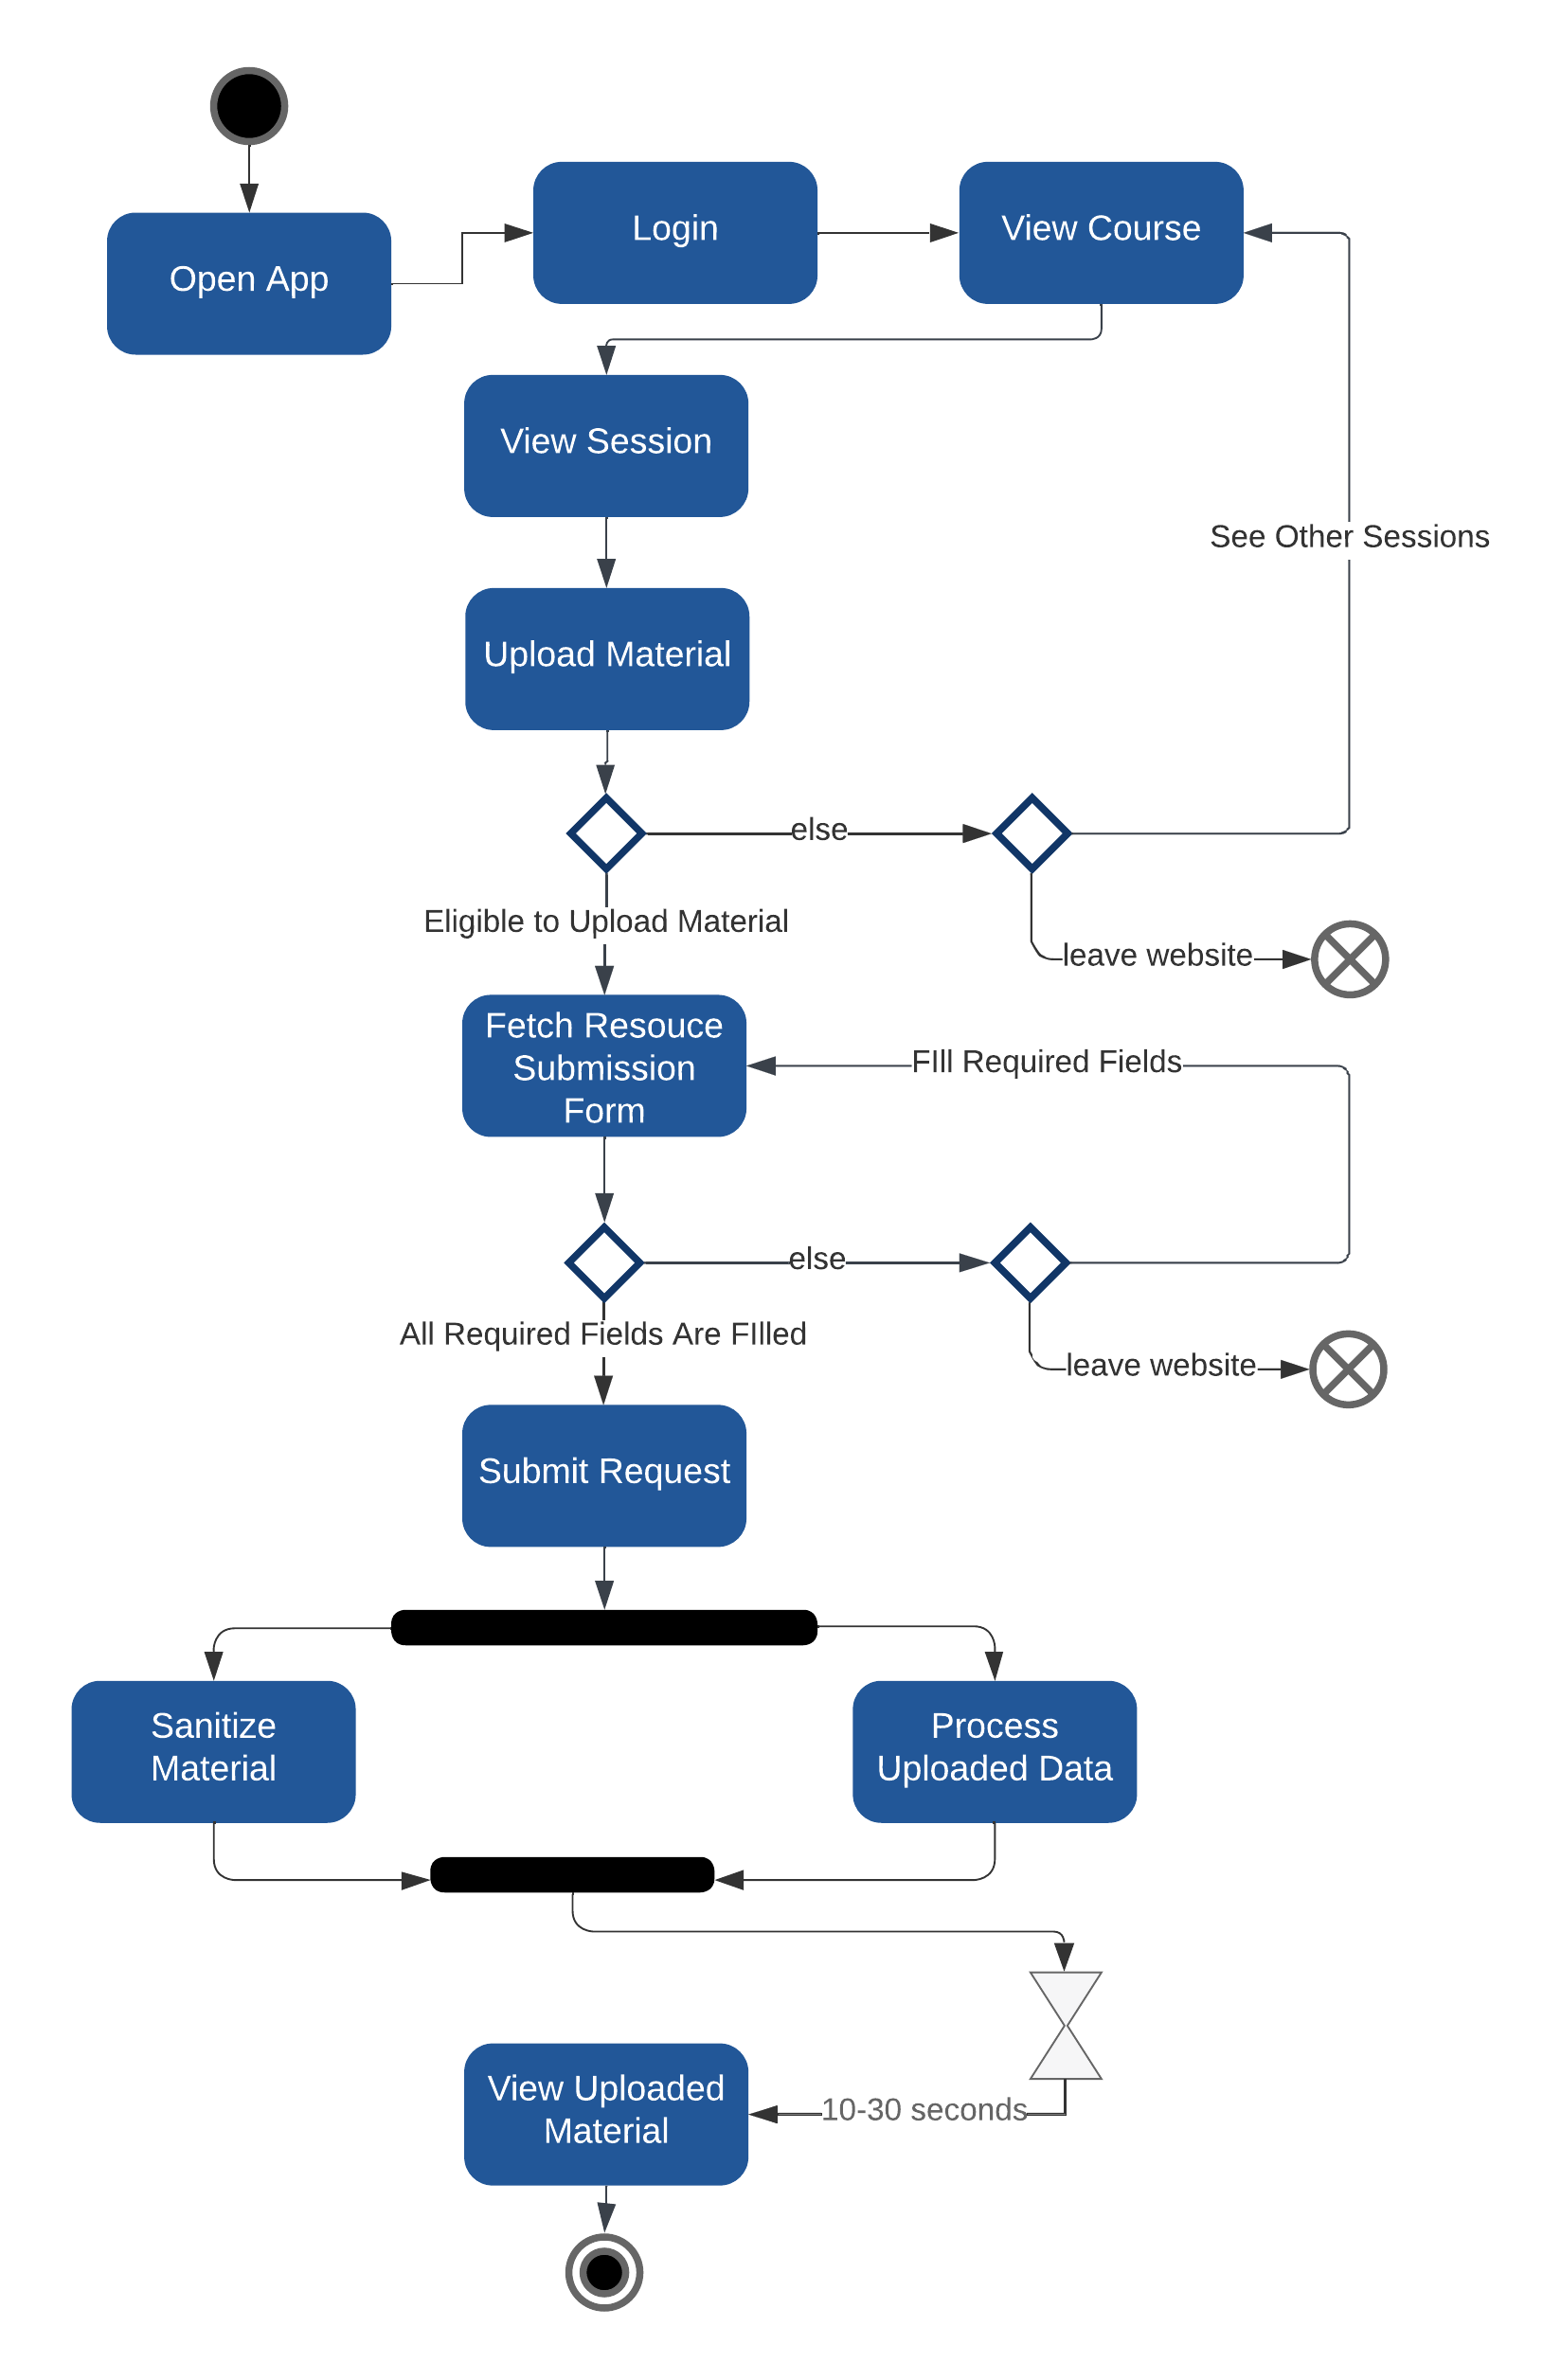
\includegraphics[width=150mm,scale=1]{figures/analysis_and_design/analysis/3. Upload Material.png}}
    \caption{Use case model - upload material}
    \label{uploadMaterial}
\end{figure}



\subsection{Requirement Validation}
\begin{justify}
\vspace{0.25cm}
The requirements validation phase is an essential step in ensuring that this software meets the needs of the end-user at STDC. This section provides an overview of the project's requirements validation procedure.

\vspace{0.25cm}
\newendline A list of the validated requirements can be found in the first section of this chapter. The list provides a high level overview of the requirements and their relationship to each other. The requirements have been validated through a combination of methods, including stakeholder meetings, inspection of existing documentation, requirements specification testing (as outlined in chapter 5, section of testing), and finite state machine analysis (also outlined in chapter 5, section of testing).

\vspace{0.25cm}
\newendline During the validation process, a number of issues and discrepancies were identified. These are shown in Figures \ref{FSM}, \ref{FSMTable}, and Appendices \pageref{Appendix 2}, which provide a detailed look at each of the issues and the steps taken to resolve them. While many of the issues required changes to the requirements, some of them have been addressed through the design and development of the system.

\vspace{0.25cm}
\newendline The overall effectiveness of the validation process has been positive, and the requirements have been deemed to be of high quality. The validation process has provided valuable feedback that has been used to improve the overall design of the system, and it has helped to ensure that the software will meet the needs of the stakeholders.

\vspace{0.25cm}
\newendline In terms of sign-off, stakeholders have been involved throughout the development process and have provided feedback and input on the requirements. While a formal sign-off is not available, their active participation and engagement in the process serves as validation and acceptance of the requirements.
\end{justify}



\clearpage
